\documentclass[11pt,german,a4paper]{article}
\usepackage[default]{sourcesanspro}
\usepackage{amssymb,amsmath,xfrac,icomma}
\usepackage{ifxetex,ifluatex}
\usepackage{fixltx2e} % provides \textsubscript
\ifnum 0\ifxetex 1\fi\ifluatex 1\fi=0 % if pdftex
  \usepackage[T1]{fontenc}
  \usepackage[utf8x]{inputenc}
\else % if luatex or xelatex
  \ifxetex
    \usepackage{mathspec}
  \else
    \usepackage{fontspec}
  \fi
  \defaultfontfeatures{Ligatures=TeX,Scale=MatchLowercase}
\fi
% use upquote if available, for straight quotes in verbatim environments
\IfFileExists{upquote.sty}{\usepackage{upquote}}{}
% use microtype if available
\IfFileExists{microtype.sty}{%
\usepackage{microtype}
\UseMicrotypeSet[protrusion]{basicmath} % disable protrusion for tt fonts
}{}

\usepackage[margin=2.5cm,top=3.5cm,bottom=3cm]{geometry}
\usepackage{hyperref}
\PassOptionsToPackage{usenames,dvipsnames}{color} % color is loaded by hyperref
\usepackage[table,dvipsnames]{xcolor}
\definecolor{goethe_blue}{HTML}{00618F}
\definecolor{light_gray}{HTML}{f8f6f5}
\definecolor{sand_gray}{HTML}{e4e3dd}
\definecolor{dark_gray}{HTML}{4d4b46}
\definecolor{purple}{HTML}{860047}
\definecolor{emo_red}{HTML}{b3062c}
\definecolor{mustard_yellow}{HTML}{e3ba0f}
\definecolor{green}{HTML}{737c45}
\definecolor{magenta}{HTML}{ad3b76}
\definecolor{orange}{HTML}{c96215}
\definecolor{sun_yellow}{HTML}{f7d926}
\definecolor{light_green}{HTML}{a5ab52}
\definecolor{light_blue}{HTML}{48a9da}
\hypersetup{unicode=true,
            colorlinks=true,
            linkcolor=goethe_blue,
            citecolor=goethe_blue,
            urlcolor=goethe_blue,
            breaklinks=true}
\urlstyle{same}  % don't use monospace font for urls
\newcommand{\lastupdate}{Stand: }
\newcommand{\pagestring}{Seite }
\ifnum 0\ifxetex 1\fi\ifluatex 1\fi=0 % if pdftex
  \usepackage[shorthands=off,main=ngerman]{babel}
\else
  \usepackage{polyglossia}
  \setmainlanguage[]{german}
\fi
\iflanguage{english}{%
  \renewcommand{\lastupdate}{Last updated }%
  \renewcommand{\pagestring}{Page }%
}{}
\usepackage{color}
\usepackage{fancyvrb}
\newcommand{\VerbBar}{|}
\newcommand{\VERB}{\Verb[commandchars=\\\{\}]}
\DefineVerbatimEnvironment{Highlighting}{Verbatim}{commandchars=\\\{\}}
% Add ',fontsize=\small' for more characters per line
\usepackage{framed}
\definecolor{shadecolor}{RGB}{248,248,248}
\newenvironment{Shaded}{\begin{snugshade}}{\end{snugshade}}
\newcommand{\AlertTok}[1]{\textcolor[rgb]{0.94,0.16,0.16}{#1}}
\newcommand{\AnnotationTok}[1]{\textcolor[rgb]{0.56,0.35,0.01}{\textbf{\textit{#1}}}}
\newcommand{\AttributeTok}[1]{\textcolor[rgb]{0.77,0.63,0.00}{#1}}
\newcommand{\BaseNTok}[1]{\textcolor[rgb]{0.00,0.00,0.81}{#1}}
\newcommand{\BuiltInTok}[1]{#1}
\newcommand{\CharTok}[1]{\textcolor[rgb]{0.31,0.60,0.02}{#1}}
\newcommand{\CommentTok}[1]{\textcolor[rgb]{0.56,0.35,0.01}{\textit{#1}}}
\newcommand{\CommentVarTok}[1]{\textcolor[rgb]{0.56,0.35,0.01}{\textbf{\textit{#1}}}}
\newcommand{\ConstantTok}[1]{\textcolor[rgb]{0.00,0.00,0.00}{#1}}
\newcommand{\ControlFlowTok}[1]{\textcolor[rgb]{0.13,0.29,0.53}{\textbf{#1}}}
\newcommand{\DataTypeTok}[1]{\textcolor[rgb]{0.13,0.29,0.53}{#1}}
\newcommand{\DecValTok}[1]{\textcolor[rgb]{0.00,0.00,0.81}{#1}}
\newcommand{\DocumentationTok}[1]{\textcolor[rgb]{0.56,0.35,0.01}{\textbf{\textit{#1}}}}
\newcommand{\ErrorTok}[1]{\textcolor[rgb]{0.64,0.00,0.00}{\textbf{#1}}}
\newcommand{\ExtensionTok}[1]{#1}
\newcommand{\FloatTok}[1]{\textcolor[rgb]{0.00,0.00,0.81}{#1}}
\newcommand{\FunctionTok}[1]{\textcolor[rgb]{0.00,0.00,0.00}{#1}}
\newcommand{\ImportTok}[1]{#1}
\newcommand{\InformationTok}[1]{\textcolor[rgb]{0.56,0.35,0.01}{\textbf{\textit{#1}}}}
\newcommand{\KeywordTok}[1]{\textcolor[rgb]{0.13,0.29,0.53}{\textbf{#1}}}
\newcommand{\NormalTok}[1]{#1}
\newcommand{\OperatorTok}[1]{\textcolor[rgb]{0.81,0.36,0.00}{\textbf{#1}}}
\newcommand{\OtherTok}[1]{\textcolor[rgb]{0.56,0.35,0.01}{#1}}
\newcommand{\PreprocessorTok}[1]{\textcolor[rgb]{0.56,0.35,0.01}{\textit{#1}}}
\newcommand{\RegionMarkerTok}[1]{#1}
\newcommand{\SpecialCharTok}[1]{\textcolor[rgb]{0.00,0.00,0.00}{#1}}
\newcommand{\SpecialStringTok}[1]{\textcolor[rgb]{0.31,0.60,0.02}{#1}}
\newcommand{\StringTok}[1]{\textcolor[rgb]{0.31,0.60,0.02}{#1}}
\newcommand{\VariableTok}[1]{\textcolor[rgb]{0.00,0.00,0.00}{#1}}
\newcommand{\VerbatimStringTok}[1]{\textcolor[rgb]{0.31,0.60,0.02}{#1}}
\newcommand{\WarningTok}[1]{\textcolor[rgb]{0.56,0.35,0.01}{\textbf{\textit{#1}}}}
\usepackage{longtable,booktabs}
\usepackage{calc} % for calculating minipage widths
% Correct order of tables after \paragraph or \subparagraph
\usepackage{etoolbox}
\makeatletter
\patchcmd\longtable{\par}{\if@noskipsec\mbox{}\fi\par}{}{}
\makeatother
% Allow footnotes in longtable head/foot
\IfFileExists{footnotehyper.sty}{\usepackage{footnotehyper}}{\usepackage{footnote}}
\makesavenoteenv{longtable}
\usepackage{graphicx,grffile}
\makeatletter
\def\maxwidth{\ifdim\Gin@nat@width>\linewidth\linewidth\else\Gin@nat@width\fi}
\def\maxheight{\ifdim\Gin@nat@height>\textheight\textheight\else\Gin@nat@height\fi}
\makeatother
% Scale images if necessary, so that they will not overflow the page
% margins by default, and it is still possible to overwrite the defaults
% using explicit options in \includegraphics[width, height, ...]{}
\setkeys{Gin}{width=\maxwidth,height=\maxheight,keepaspectratio}
\usepackage[normalem]{ulem}
% avoid problems with \sout in headers with hyperref:
\pdfstringdefDisableCommands{\renewcommand{\sout}{}}
\IfFileExists{parskip.sty}{%
\usepackage{parskip}
}{% else
\setlength{\parindent}{0pt}
\setlength{\parskip}{6pt plus 2pt minus 1pt}
}
\setlength{\emergencystretch}{3em}  % prevent overfull lines
\providecommand{\tightlist}{%
  \setlength{\itemsep}{0pt}\setlength{\parskip}{0pt}}
\setcounter{secnumdepth}{5}
% Redefines (sub)paragraphs to behave more like sections
\ifx\paragraph\undefined\else
\let\oldparagraph\paragraph
\renewcommand{\paragraph}[1]{\oldparagraph{#1}\mbox{}}
\fi
\ifx\subparagraph\undefined\else
\let\oldsubparagraph\subparagraph
\renewcommand{\subparagraph}[1]{\oldsubparagraph{#1}\mbox{}}
\fi

%%% Use protect on footnotes to avoid problems with footnotes in titles
\let\rmarkdownfootnote\footnote%
\def\footnote{\protect\rmarkdownfootnote}

%%% Change title format to be more compact
\usepackage{titling}

% Create subtitle command for use in maketitle
\newcommand{\subtitle}[1]{
  \posttitle{
    \begin{center}\large#1\end{center}
    }
}

\setlength{\droptitle}{-2em}
  \title{Spatial Analysis mit R (I)}
  \pretitle{\vspace{\droptitle}\centering\huge}
  \posttitle{\par}
\subtitle{Methodenwoche}
  \author{true}
  \preauthor{\centering\large\emph}
  \postauthor{\par}
  \predate{\centering\large\emph}
  \postdate{\par}
  \date{20.--21. September 2021}


% required by kableextra %
\usepackage{booktabs}
\usepackage{longtable}
\usepackage{array}
\usepackage{multirow}
\usepackage{wrapfig}
\usepackage{float}
\usepackage{colortbl}
\usepackage{pdflscape}
\usepackage{tabu}
\usepackage{threeparttable}
\usepackage[normalem]{ulem}

% custom %
\usepackage{icomma}
\usepackage{fancyhdr}
\usepackage{lastpage}
\usepackage{multicol}


\usepackage{tcolorbox}
%\newtcolorbox{rtip}{colframe=purple,colback=light_gray,title=Softwarehinweis}
\newenvironment{rtip}{
  \medskip
  \begin{tcolorbox}[colframe=purple,colback=light_gray,title=Softwarehinweis]
}{
  \end{tcolorbox}
  \medskip
}

\usepackage{csquotes}
\usepackage{gensymb}
\usepackage{makecell}
\usepackage{tabularx}
\usepackage{arydshln}
\usepackage{caption}
\usepackage{bbding}

\pagestyle{fancy}
\fancyhf{}
\usepackage{xpatch}
\xpretocmd\headrule{\color{dark_gray}}{}{\PatchFailed}
\lhead{\color{dark_gray}\footnotesize Spatial Analysis mit R (I)}
\chead{\color{dark_gray}\footnotesize }
\rhead{\color{dark_gray}\footnotesize Methodenwoche}
  \lfoot{\color{dark_gray}\footnotesize\lastupdate\today}
\rfoot{\color{dark_gray}\footnotesize\pagestring\thepage/\begin{NoHyper}\pageref{LastPage}\end{NoHyper}}
\fancypagestyle{plain}{ %
  \fancyhf{} % remove everything
  \renewcommand{\headrulewidth}{0pt} % remove lines as well
  \renewcommand{\footrulewidth}{0pt}
      \lfoot{\color{dark_gray}\footnotesize\lastupdate\today}
    \rfoot{\color{dark_gray}\footnotesize\pagestring\thepage/\begin{NoHyper}\pageref{LastPage}\end{NoHyper}}
}
\renewcommand{\maketitle}{
  \newpage
  \begingroup
    \setlength{\parindent}{0pt}
    \setlength{\parskip}{4pt}
    {\fontseries{b}\selectfont\Huge{Spatial Analysis mit R (I)}\par}
    {\fontseries{l}\LARGE{Methodenwoche}\par\bigskip}

    \bigskip

    \begin{tabularx}{\textwidth}{@{}X r}
                  Till Straube
        \newline \href{mailto:straube@geo.uni-frankfurt.de}{\nolinkurl{straube@geo.uni-frankfurt.de}}
                  \medskip\newline
          {\renewcommand\\{\newline}Institut für Humangeographie\\
Goethe-Universität Frankfurt}
         &
                    20.--21. September 2021
        \end{tabularx}
  \endgroup
  \vspace{1.1cm}
  \thispagestyle{plain}% suppress the running head
}

\newcommand{\makenotation}{
  \begin{center}
    \fontseries{l}\selectfont
    \huge  
  \end{center}
  \bigskip
}

\newcommand{\divider}{
  \medskip
  \begin{center}
  {\color{orange}\SparkleBold}
  \end{center}
  \medskip
}


\makeatletter
\renewcommand{\@listI}{%
\leftmargin=25pt
\rightmargin=0pt
\labelsep=5pt
\labelwidth=20pt
\itemindent=0pt
\listparindent=0pt
\topsep=0pt plus 2pt minus 4pt
\partopsep=0pt plus 1pt minus 1pt
\parsep=3pt plus 1pt minus 1pt
\itemsep=\parsep}
\makeatother

\begin{document}
\maketitle

{
\setcounter{tocdepth}{2}
\tableofcontents
}
\hypertarget{zeitplan}{%
\section*{Zeitplan}\label{zeitplan}}
\addcontentsline{toc}{section}{Zeitplan}

Alle Sitzungen finden über Zoom statt.

\begin{longtable}[]{@{}
  >{\raggedright\arraybackslash}p{(\columnwidth - 4\tabcolsep) * \real{0.1667}}
  >{\raggedright\arraybackslash}p{(\columnwidth - 4\tabcolsep) * \real{0.4167}}
  >{\raggedright\arraybackslash}p{(\columnwidth - 4\tabcolsep) * \real{0.4167}}@{}}
\toprule
\begin{minipage}[b]{\linewidth}\raggedright
Zeit
\end{minipage} & \begin{minipage}[b]{\linewidth}\raggedright
Montag
\end{minipage} & \begin{minipage}[b]{\linewidth}\raggedright
Dienstag
\end{minipage} \\
\midrule
\endhead
10:00--11:30 & \textbf{(1) \protect\hyperlink{getting-started}{Getting started} (LAS)} & \textbf{(5) Geodaten verschneiden: FTR} \\
\emph{11:30--11:45} & \emph{Kaffeepause} & \emph{Kaffeepause} \\
11:45--13:15 & \textbf{(2) \protect\hyperlink{daten-visualisieren}{Daten visualisieren} (FTR, HOS)} & \textbf{(6) Geodaten verschneiden: HOS, SYW} \\
\emph{13:15--14:15} & \emph{Mittagspause} & \emph{Mittagspause} \\
14:15--15:45 & \textbf{(3) \protect\hyperlink{karten-erstellen-ftr}{Karten erstellen} (FTR)} & \textbf{(7) Nach Hilfe fragen und und publizieren (FTR)} \\
\emph{15:45--16:15} & \emph{Kaffeepause} & \emph{Kaffeepause} \\
16:15--18:00 & \textbf{(4) \protect\hyperlink{karten-erstellen-hos}{Karten erstellen} (HOS, SYW)} & \textbf{(8) Looking back, looking ahead (LAS)} \\
\bottomrule
\end{longtable}

\hypertarget{getting-started}{%
\section{Getting started}\label{getting-started}}

\hypertarget{formales}{%
\subsection{Formales}\label{formales}}

\hypertarget{keine-reguluxe4re-anrechnung-des-workshops}{%
\subsubsection{Keine reguläre Anrechnung des Workshops}\label{keine-reguluxe4re-anrechnung-des-workshops}}

\begin{itemize}
\tightlist
\item
  Die Methodenwoche ist eine außercurriculare Veranstaltung
\item
  Keine Anrechnung als Prüfungsleistung für das reguläre Studium
\item
  Alle Teilnehmer*innen erhalten Methodenzentrum eine Bescheinigung über die erbrachte Leistung (Ende 2021/Anfang 2022)
\end{itemize}

\hypertarget{methodenzertifikat}{%
\subsubsection{Methodenzertifikat}\label{methodenzertifikat}}

\begin{itemize}
\tightlist
\item
  Nur für Bachelor-Studierende der Fachbereiche 02--05
\item
  Kann mit 5 CP beantragt werden
\item
  z.~B. Teilnahme Workshop (2 CP) + Leistungsnachweis (3 CP)
\item
  Maximal 20\% Fehlzeit zulässig für Teilnahmenachweis
\item
  Schriftliche Leistungsnachweise mit maximal vierwöchiger Abgabefrist
\item
  Alle Fragen dazu bitte an \href{mailto:hiwis-methodenzentrum@uni-frankfurt.de}{\nolinkurl{hiwis-methodenzentrum@uni-frankfurt.de}}
\end{itemize}

\hypertarget{leistungsnachweis}{%
\subsubsection{Leistungsnachweis}\label{leistungsnachweis}}

\begin{itemize}
\tightlist
\item
  Schriftliche Ausarbeitung
\item
  In Form eines kleinen Forschungsberichts:

  \begin{itemize}
  \tightlist
  \item
    Thematische Einleitung
  \item
    Fragestellung
  \item
    Beschreibung der Datenquelle(n)
  \item
    Nachvollziehbare Bearbeitung der Daten
  \item
    Nachvollziehbare Visualisierung(en)
  \item
    Interpretation
  \end{itemize}
\item
  Format: Rmarkdown + (Roh-)datensatz
\end{itemize}

\hypertarget{inhaltliches}{%
\subsection{Inhaltliches}\label{inhaltliches}}

\hypertarget{lernziele-der-veranstaltung}{%
\subsubsection{Lernziele der Veranstaltung}\label{lernziele-der-veranstaltung}}

Sie können\ldots{}

\begin{itemize}
\tightlist
\item
  Datenvisualisierungen nachvollziehen und selbst gestalten.
\item
  Geodaten einlesen, transformieren und verschneiden.
\item
  Geodaten kartographisch darstellen.
\item
  Reproducible examples erstellen um nach Hilfe zu fragen.
\item
  Berichte in Rmarkdown verfassen und rendern.
\end{itemize}

\hypertarget{seminarkonzept}{%
\subsubsection{Seminarkonzept}\label{seminarkonzept}}

\begin{itemize}
\tightlist
\item
  Kompetenter Umgang mit Geodaten als Kernziel
\item
  Aber nicht im luftleeren Raum
\item
  Das Drumherum ist mindestens genauso wichtig
\item
  Unterlagen sind Auszüge aus einem zweisemestrigen Seminar
\end{itemize}

\hypertarget{opinionated}{%
\subsubsection{\texorpdfstring{``Opinionated\ldots{}''}{``Opinionated\ldots''}}\label{opinionated}}

\begin{itemize}
\tightlist
\item
  package choices:

  \begin{itemize}
  \tightlist
  \item
    \texttt{tidyverse}
  \item
    \texttt{sf}
  \end{itemize}
\item
  coding style:

  \begin{itemize}
  \tightlist
  \item
    Functional
  \item
    Pipes \texttt{\%\textgreater{}\%}
  \end{itemize}
\item
  workflow:

  \begin{itemize}
  \tightlist
  \item
    Incremental commands
  \item
    Rmarkdown (reproducible research)
  \end{itemize}
\end{itemize}

\hypertarget{didaktisches}{%
\subsection{Didaktisches}\label{didaktisches}}

\hypertarget{herausforderungen-in-der-it-didaktik}{%
\subsubsection{Herausforderungen in der IT-Didaktik}\label{herausforderungen-in-der-it-didaktik}}

\begin{itemize}
\tightlist
\item
  Unterschiedliche Erfahrungen, Kompetenzen und Herangehensweisen
\item
  Die eine Hälfte versteht gar nichts, die andere langweilt sich
\item
  Kleinster gemeinsamer Nenner: Schritt-für-Schritt-Anleitungen
\item
  In der Praxis wertlos
\end{itemize}

\hypertarget{everyone-fails}{%
\subsubsection{Everyone fails}\label{everyone-fails}}

\begin{itemize}
\tightlist
\item
  In der Praxis stoßen alle ständig an die Grenzen ihrer technischen Kompetenz.
\item
  Es geht darum, sich am Limit einigermaßen wohl zu fühlen und die Grenzen zu verschieben.
\item
  Gute Angewohnheiten (Strukturen, Formate, Stil) helfen dabei!
\end{itemize}

\hypertarget{mein-ansatz-in-der-lehre}{%
\subsubsection{Mein Ansatz in der Lehre}\label{mein-ansatz-in-der-lehre}}

\begin{itemize}
\tightlist
\item
  Strategische Überforderung durch schwierige Aufgaben?
\item
  Lösungsorientierte Didaktik!
\item
  Die affektive Seite (Spaß, Frust) ernst nehmen und thematisieren
\item
  Frustrationsschwelle trainieren
\end{itemize}

\hypertarget{schattenkompetenzen}{%
\subsubsection{``Schattenkompetenzen''}\label{schattenkompetenzen}}

\begin{itemize}
\tightlist
\item
  Über Code reden
\item
  Fehlermeldungen lesen
\item
  Gezielt googlen (und Antworten auswählen)
\item
  Copy, paste, customize
\item
  Gute Fragen (online) stellen
\end{itemize}

\hypertarget{dieser-workshop-findet-in-verschiedenen-modi-statt}{%
\subsubsection{Dieser Workshop findet in verschiedenen Modi statt:}\label{dieser-workshop-findet-in-verschiedenen-modi-statt}}

\hypertarget{listen-and-share-las}{%
\paragraph{Listen and share (LAS)}\label{listen-and-share-las}}

\begin{itemize}
\tightlist
\item
  Ich rede (mit Folien oder ohne) oder moderiere eine Diskussion.
\item
  Sie hören mir und Ihren Kommiliton*innen aufmerksam zu.
\item
  Sie ``melden'' sich für Redebeiträge oder Fragen (Zoom-Funktion).
\end{itemize}

\hypertarget{follow-the-recipe-ftr}{%
\paragraph{Follow the recipe (FTR)}\label{follow-the-recipe-ftr}}

\begin{itemize}
\tightlist
\item
  Ich teile ein unvollständiges Beispielprojekt.
\item
  Wir gehen die Teilschritte nach und nach durch.
\item
  Ich ``habe den Plan'', stelle aber immer wieder Fragen ans Plenum.
\item
  Sie vollziehen die Schritte an Ihrer eigenen Kopie des Projekts nach.
\item
  Sie unterbrechen mich mit Nachfragen oder Problemen.
\end{itemize}

\hypertarget{hands-on-session-hos}{%
\paragraph{Hands-on session (HOS)}\label{hands-on-session-hos}}

\begin{itemize}
\tightlist
\item
  Sie bearbeiten praktische Aufgabenstellungen alleine.
\item
  Dabei sind sie in zufälligen Dreier-Konstellationen (Breakout-Session).
\item
  Bei Fragen oder Problemen wenden Sie sich zunächst an Ihre Kleingruppe.
\item
  Falls Sie nicht weiterkommen, fordern Sie Hilfe an (Zoom-Funktion).
\item
  Ich reagiere auf Hilfegesuche oder ``mache die Runde''.
\end{itemize}

\hypertarget{share-your-work-syw}{%
\paragraph{Share your work (SYW)}\label{share-your-work-syw}}

\begin{itemize}
\tightlist
\item
  Ich wähle eine Teilnehmer*in zufällig aus.
\item
  Die Person teilt ihren Bildschirm und berichtet von ihrer Bearbeitung eines Problems.
\item
  Alle anderen unterstützen solidarisch durch aktives Nachvollziehen, Nachfragen und Hinweise.
\end{itemize}

\hypertarget{technisches}{%
\subsection{Technisches}\label{technisches}}

\hypertarget{arbeitsplatz}{%
\subsubsection{Arbeitsplatz}\label{arbeitsplatz}}

\begin{itemize}
\tightlist
\item
  Challenge: Zoom (meinen Bildschirm) und R gleichzeitig sehen
\item
  Am allerbesten: Zweiter Bildschirm
\item
  Auch gut: Zweites Gerät (Tablet)
\end{itemize}

\hypertarget{workshopunterlagen}{%
\subsubsection{Workshopunterlagen}\label{workshopunterlagen}}

\begin{itemize}
\tightlist
\item
  Bookdown (statt OLAT)
\item
  \sout{Können} Werden sich verändern
\item
  Am besten neu laden mit Strg+Umschalt+R
\item
  \url{https://tiny.gu/mwsa}
\end{itemize}

\hypertarget{rstudio-cloud}{%
\subsubsection{RStudio Cloud}\label{rstudio-cloud}}

\begin{itemize}
\tightlist
\item
  Grundsätzliche Empfehlung: R und RStudio lokal installieren
\item
  Wir nutzen im Rahmen des Workshops die RStudio Cloud

  \begin{itemize}
  \tightlist
  \item
    für einfaches Teilen von Code
  \item
    für ein homogenes Setup
  \end{itemize}
\end{itemize}

\hypertarget{daten-visualisieren}{%
\section{Daten visualisieren}\label{daten-visualisieren}}

\hypertarget{lernziele-dieser-sitzung}{%
\subsection{Lernziele dieser Sitzung}\label{lernziele-dieser-sitzung}}

Sie können\ldots{}

\begin{itemize}
\tightlist
\item
  einfache Befehle zur Visualisierung in Base R anwenden.
\item
  die Grammatik von \texttt{ggplot2} für Visualisierungen in Grundzügen wiedergeben und anwenden.
\item
  eigene Ideen für Visualisierungen entwickeln und umsetzen.
\end{itemize}

\hypertarget{voraussetzungen}{%
\subsection{Voraussetzungen}\label{voraussetzungen}}

Für diese Lektion benötigen wir das Paket \texttt{tidyverse}:

\begin{Shaded}
\begin{Highlighting}[]
\FunctionTok{library}\NormalTok{(tidyverse)}
\end{Highlighting}
\end{Shaded}

Und einen Datensatz, der in Form eines tibble vorliegt. Der Beispieldatensatz \texttt{diamonds} wird mitgeliefert:

\begin{Shaded}
\begin{Highlighting}[]
\NormalTok{diamonds}
\DocumentationTok{\#\# \# A tibble: 53,940 x 10}
\DocumentationTok{\#\#    carat cut       color clarity depth table price     x     y     z}
\DocumentationTok{\#\#    \textless{}dbl\textgreater{} \textless{}ord\textgreater{}     \textless{}ord\textgreater{} \textless{}ord\textgreater{}   \textless{}dbl\textgreater{} \textless{}dbl\textgreater{} \textless{}int\textgreater{} \textless{}dbl\textgreater{} \textless{}dbl\textgreater{} \textless{}dbl\textgreater{}}
\DocumentationTok{\#\#  1  0.23 Ideal     E     SI2      61.5    55   326  3.95  3.98  2.43}
\DocumentationTok{\#\#  2  0.21 Premium   E     SI1      59.8    61   326  3.89  3.84  2.31}
\DocumentationTok{\#\#  3  0.23 Good      E     VS1      56.9    65   327  4.05  4.07  2.31}
\DocumentationTok{\#\#  4  0.29 Premium   I     VS2      62.4    58   334  4.2   4.23  2.63}
\DocumentationTok{\#\#  5  0.31 Good      J     SI2      63.3    58   335  4.34  4.35  2.75}
\DocumentationTok{\#\#  6  0.24 Very Good J     VVS2     62.8    57   336  3.94  3.96  2.48}
\DocumentationTok{\#\#  7  0.24 Very Good I     VVS1     62.3    57   336  3.95  3.98  2.47}
\DocumentationTok{\#\#  8  0.26 Very Good H     SI1      61.9    55   337  4.07  4.11  2.53}
\DocumentationTok{\#\#  9  0.22 Fair      E     VS2      65.1    61   337  3.87  3.78  2.49}
\DocumentationTok{\#\# 10  0.23 Very Good H     VS1      59.4    61   338  4     4.05  2.39}
\DocumentationTok{\#\# \# ... with 53,930 more rows}
\end{Highlighting}
\end{Shaded}

Wenn wir mögen, können wir ihn mit der Funktion \texttt{data()} explizit in unser Environment laden:

\begin{Shaded}
\begin{Highlighting}[]
\FunctionTok{data}\NormalTok{(diamonds)}
\end{Highlighting}
\end{Shaded}

\hypertarget{uxfcberblick}{%
\subsection{Überblick}\label{uxfcberblick}}

Einen ersten Überblick kriegen wir zum Einen durch den Befehl \texttt{str()}, der uns die Typen in den Spalten anzeigt:

\begin{Shaded}
\begin{Highlighting}[]
\FunctionTok{str}\NormalTok{(diamonds)}
\DocumentationTok{\#\# tibble [53,940 x 10] (S3: tbl\_df/tbl/data.frame)}
\DocumentationTok{\#\#  $ carat  : num [1:53940] 0.23 0.21 0.23 0.29 0.31 0.24 0.24 0.26 0.22 0.23 ...}
\DocumentationTok{\#\#  $ cut    : Ord.factor w/ 5 levels "Fair"\textless{}"Good"\textless{}..: 5 4 2 4 2 3 3 3 1 3 ...}
\DocumentationTok{\#\#  $ color  : Ord.factor w/ 7 levels "D"\textless{}"E"\textless{}"F"\textless{}"G"\textless{}..: 2 2 2 6 7 7 6 5 2 5 ...}
\DocumentationTok{\#\#  $ clarity: Ord.factor w/ 8 levels "I1"\textless{}"SI2"\textless{}"SI1"\textless{}..: 2 3 5 4 2 6 7 3 4 5 ...}
\DocumentationTok{\#\#  $ depth  : num [1:53940] 61.5 59.8 56.9 62.4 63.3 62.8 62.3 61.9 65.1 59.4 ...}
\DocumentationTok{\#\#  $ table  : num [1:53940] 55 61 65 58 58 57 57 55 61 61 ...}
\DocumentationTok{\#\#  $ price  : int [1:53940] 326 326 327 334 335 336 336 337 337 338 ...}
\DocumentationTok{\#\#  $ x      : num [1:53940] 3.95 3.89 4.05 4.2 4.34 3.94 3.95 4.07 3.87 4 ...}
\DocumentationTok{\#\#  $ y      : num [1:53940] 3.98 3.84 4.07 4.23 4.35 3.96 3.98 4.11 3.78 4.05 ...}
\DocumentationTok{\#\#  $ z      : num [1:53940] 2.43 2.31 2.31 2.63 2.75 2.48 2.47 2.53 2.49 2.39 ...}
\end{Highlighting}
\end{Shaded}

Zum Anderen gibt die Hilfefunktion Auskunft über den Datensatz und die einzelnen Variablen (Metadaten):

\begin{Shaded}
\begin{Highlighting}[]
\NormalTok{?diamonds}
\end{Highlighting}
\end{Shaded}

Einen Überblick über die wichtigsten statistischen Parameter erhalten wir mit:

\begin{Shaded}
\begin{Highlighting}[]
\FunctionTok{summary}\NormalTok{(diamonds)}
\DocumentationTok{\#\#      carat               cut        color        clarity          depth      }
\DocumentationTok{\#\#  Min.   :0.2000   Fair     : 1610   D: 6775   SI1    :13065   Min.   :43.00  }
\DocumentationTok{\#\#  1st Qu.:0.4000   Good     : 4906   E: 9797   VS2    :12258   1st Qu.:61.00  }
\DocumentationTok{\#\#  Median :0.7000   Very Good:12082   F: 9542   SI2    : 9194   Median :61.80  }
\DocumentationTok{\#\#  Mean   :0.7979   Premium  :13791   G:11292   VS1    : 8171   Mean   :61.75  }
\DocumentationTok{\#\#  3rd Qu.:1.0400   Ideal    :21551   H: 8304   VVS2   : 5066   3rd Qu.:62.50  }
\DocumentationTok{\#\#  Max.   :5.0100                     I: 5422   VVS1   : 3655   Max.   :79.00  }
\DocumentationTok{\#\#                                     J: 2808   (Other): 2531                  }
\DocumentationTok{\#\#      table           price             x                y         }
\DocumentationTok{\#\#  Min.   :43.00   Min.   :  326   Min.   : 0.000   Min.   : 0.000  }
\DocumentationTok{\#\#  1st Qu.:56.00   1st Qu.:  950   1st Qu.: 4.710   1st Qu.: 4.720  }
\DocumentationTok{\#\#  Median :57.00   Median : 2401   Median : 5.700   Median : 5.710  }
\DocumentationTok{\#\#  Mean   :57.46   Mean   : 3933   Mean   : 5.731   Mean   : 5.735  }
\DocumentationTok{\#\#  3rd Qu.:59.00   3rd Qu.: 5324   3rd Qu.: 6.540   3rd Qu.: 6.540  }
\DocumentationTok{\#\#  Max.   :95.00   Max.   :18823   Max.   :10.740   Max.   :58.900  }
\DocumentationTok{\#\#                                                                   }
\DocumentationTok{\#\#        z         }
\DocumentationTok{\#\#  Min.   : 0.000  }
\DocumentationTok{\#\#  1st Qu.: 2.910  }
\DocumentationTok{\#\#  Median : 3.530  }
\DocumentationTok{\#\#  Mean   : 3.539  }
\DocumentationTok{\#\#  3rd Qu.: 4.040  }
\DocumentationTok{\#\#  Max.   :31.800  }
\DocumentationTok{\#\# }
\end{Highlighting}
\end{Shaded}

\hypertarget{visualisierung-mit-dem-standardpaket}{%
\subsection{Visualisierung mit dem Standardpaket}\label{visualisierung-mit-dem-standardpaket}}

Es gibt in R mehrere grundlegend verschiedene Möglichkeiten, Daten zu visualisieren. Für einen schnellen Überblick sind z.B. \texttt{hist()} und \texttt{boxplot()} hilfreich:

\begin{Shaded}
\begin{Highlighting}[]
\FunctionTok{hist}\NormalTok{(diamonds}\SpecialCharTok{$}\NormalTok{price)}
\end{Highlighting}
\end{Shaded}

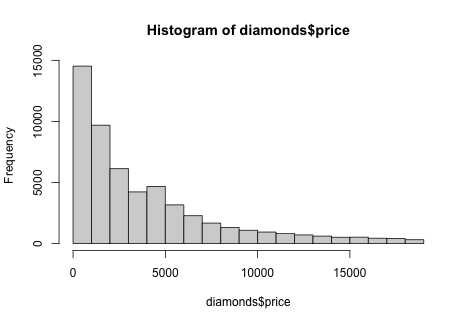
\includegraphics{_main_files/figure-latex/unnamed-chunk-9-1.png}

\begin{Shaded}
\begin{Highlighting}[]
\FunctionTok{boxplot}\NormalTok{(diamonds}\SpecialCharTok{$}\NormalTok{x)}
\end{Highlighting}
\end{Shaded}


\includegraphics{_main_files/figure-latex/unnamed-chunk-10-1.png}

\hypertarget{visualisierung-mit-ggplot}{%
\subsection{\texorpdfstring{Visualisierung mit \texttt{ggplot()}}{Visualisierung mit ggplot()}}\label{visualisierung-mit-ggplot}}

Das Paket \texttt{ggplot2} ist Teil vom \texttt{tidyverse}. Hiermit lassen sich sehr flexible Graphiken gestalten. Wir werden ausschließlich mit diesem System arbeiten.

Die Syntax ist dabei auf den ersten Blick etwas komplexer.

Am Anfang steht der Befehl \texttt{ggplot(x)} mit dem Datensatz als Parameter

\begin{Shaded}
\begin{Highlighting}[]
\FunctionTok{ggplot}\NormalTok{(}\AttributeTok{data =}\NormalTok{ diamonds)}
\end{Highlighting}
\end{Shaded}

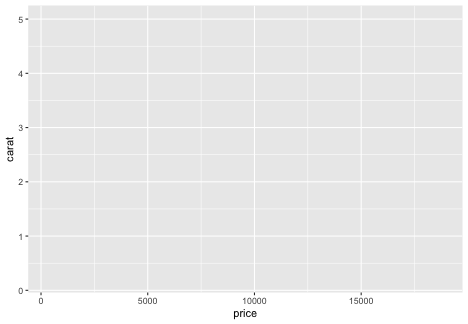
\includegraphics{_main_files/figure-latex/unnamed-chunk-11-1.png}

Mit einem Mapping-Parameter legen wir die Dimensionen fest:

\begin{Shaded}
\begin{Highlighting}[]
\FunctionTok{ggplot}\NormalTok{(}\AttributeTok{data =}\NormalTok{ diamonds, }\AttributeTok{mapping =} \FunctionTok{aes}\NormalTok{(}\AttributeTok{x =}\NormalTok{ price, }\AttributeTok{y =}\NormalTok{ carat))}
\end{Highlighting}
\end{Shaded}

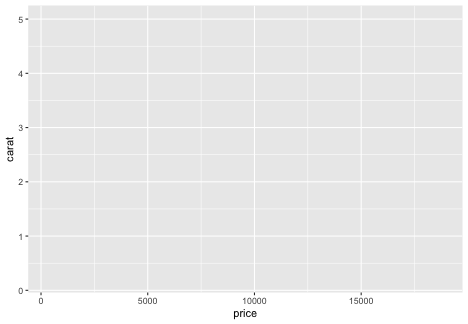
\includegraphics{_main_files/figure-latex/unnamed-chunk-12-1.png}

Das gleiche ohne Parameternamen:

\begin{Shaded}
\begin{Highlighting}[]
\FunctionTok{ggplot}\NormalTok{(diamonds, }\FunctionTok{aes}\NormalTok{(price, carat))}
\end{Highlighting}
\end{Shaded}

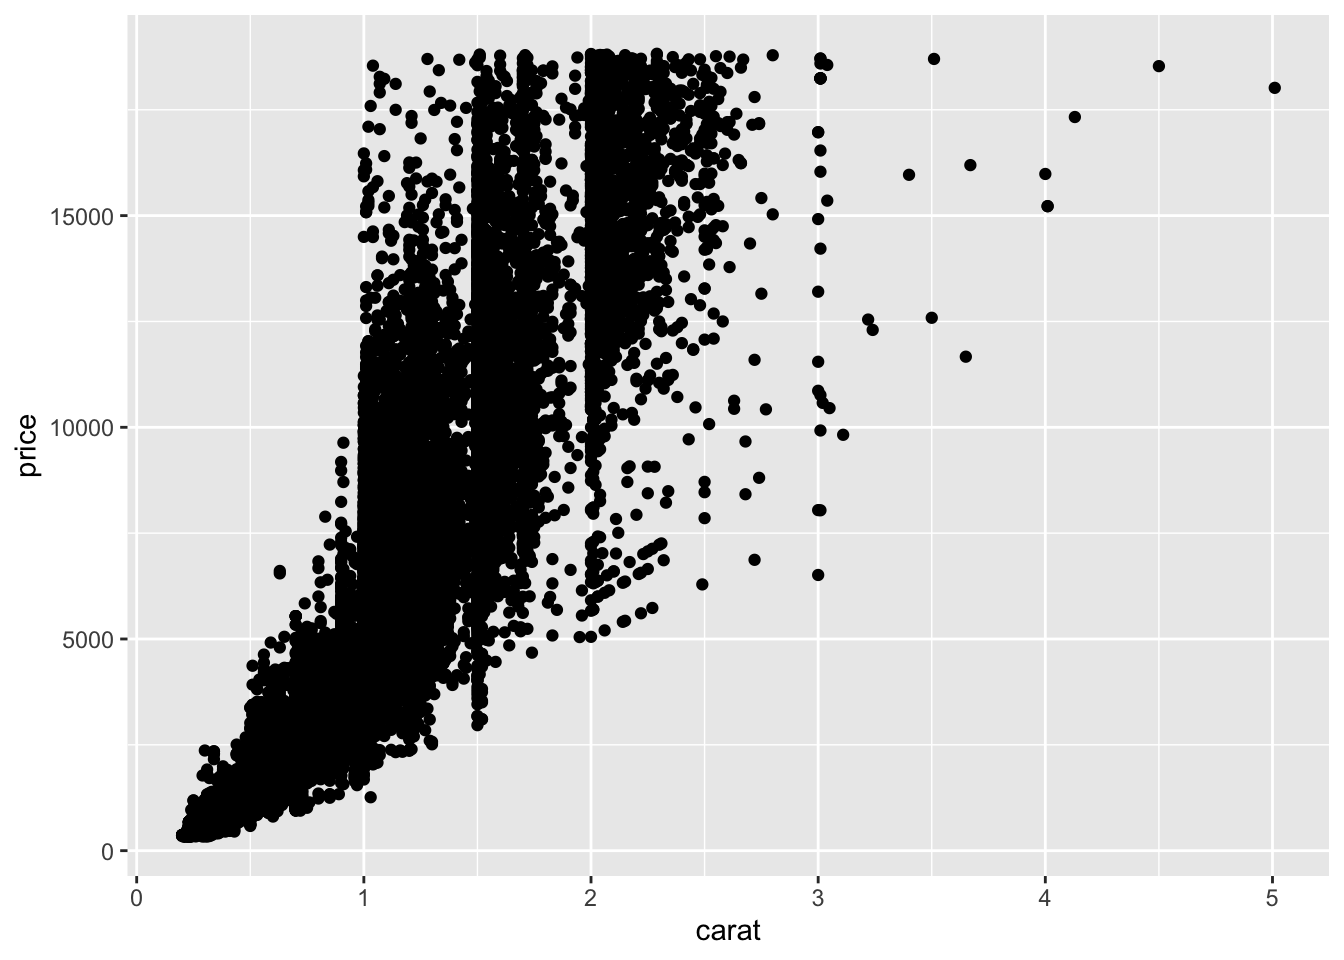
\includegraphics{_main_files/figure-latex/unnamed-chunk-13-1.png}

Nun kann mit dem \texttt{+}-Operator ein ``geometrischer'' Layer hinzugefügt werden:

\begin{Shaded}
\begin{Highlighting}[]
\FunctionTok{ggplot}\NormalTok{(diamonds, }\FunctionTok{aes}\NormalTok{(}\AttributeTok{x =}\NormalTok{ carat, }\AttributeTok{y =}\NormalTok{ price)) }\SpecialCharTok{+}
  \FunctionTok{geom\_point}\NormalTok{()}
\end{Highlighting}
\end{Shaded}

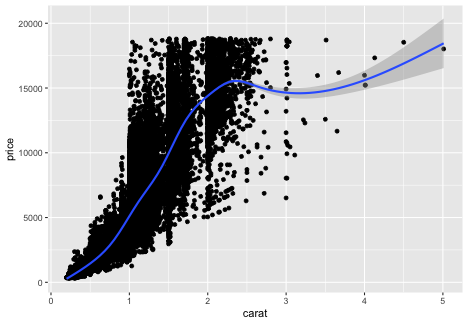
\includegraphics{_main_files/figure-latex/unnamed-chunk-14-1.png}

Weitere \texttt{geom}-Layer lassen sich mit dem \texttt{+}-Operator hinzufügen:

\begin{Shaded}
\begin{Highlighting}[]
\FunctionTok{ggplot}\NormalTok{(diamonds, }\FunctionTok{aes}\NormalTok{(}\AttributeTok{x =}\NormalTok{ carat, }\AttributeTok{y =}\NormalTok{ price)) }\SpecialCharTok{+}
  \FunctionTok{geom\_point}\NormalTok{() }\SpecialCharTok{+}
  \FunctionTok{geom\_smooth}\NormalTok{()}
\end{Highlighting}
\end{Shaded}

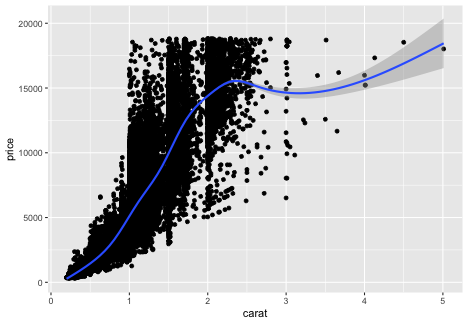
\includegraphics{_main_files/figure-latex/unnamed-chunk-15-1.png}

Die Layer-Funktionen können durch Parameter angepasst werden:

\begin{Shaded}
\begin{Highlighting}[]
\FunctionTok{ggplot}\NormalTok{(diamonds, }\FunctionTok{aes}\NormalTok{(}\AttributeTok{x =}\NormalTok{ carat, }\AttributeTok{y =}\NormalTok{ price)) }\SpecialCharTok{+}
  \FunctionTok{geom\_point}\NormalTok{(}\AttributeTok{size =} \FloatTok{0.5}\NormalTok{) }\SpecialCharTok{+}
  \FunctionTok{geom\_smooth}\NormalTok{(}\AttributeTok{color =} \StringTok{"red"}\NormalTok{)}
\end{Highlighting}
\end{Shaded}

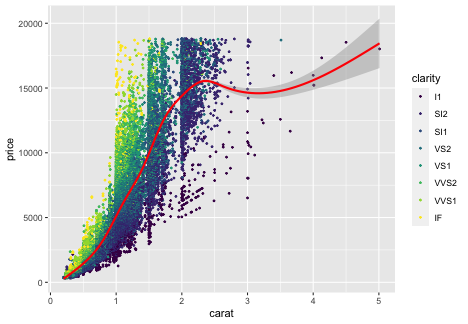
\includegraphics{_main_files/figure-latex/unnamed-chunk-16-1.png}

Dabei lassen sich in den einzelnen Layers mappings hinzufügen oder verändern:

\begin{Shaded}
\begin{Highlighting}[]
\FunctionTok{ggplot}\NormalTok{(diamonds, }\FunctionTok{aes}\NormalTok{(}\AttributeTok{x =}\NormalTok{ carat, }\AttributeTok{y =}\NormalTok{ price)) }\SpecialCharTok{+}
  \FunctionTok{geom\_point}\NormalTok{(}\FunctionTok{aes}\NormalTok{(}\AttributeTok{color =}\NormalTok{ clarity), }\AttributeTok{size =} \FloatTok{0.5}\NormalTok{) }\SpecialCharTok{+}
  \FunctionTok{geom\_smooth}\NormalTok{(}\AttributeTok{color =} \StringTok{"red"}\NormalTok{)}
\end{Highlighting}
\end{Shaded}

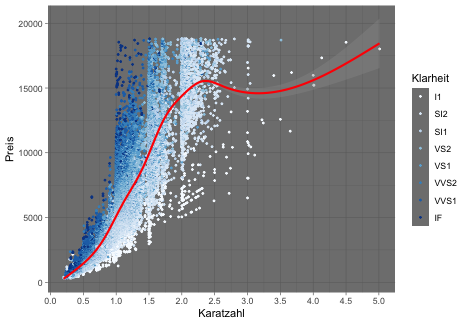
\includegraphics{_main_files/figure-latex/unnamed-chunk-17-1.png}

Schließlich lassen sich noch viele weitere optische Aspekte anpassen, z.B. Achsen, Farben, etc.:

\begin{Shaded}
\begin{Highlighting}[]
\FunctionTok{ggplot}\NormalTok{(diamonds, }\FunctionTok{aes}\NormalTok{(}\AttributeTok{x =}\NormalTok{ carat, }\AttributeTok{y =}\NormalTok{ price)) }\SpecialCharTok{+}
  \FunctionTok{geom\_point}\NormalTok{(}\FunctionTok{aes}\NormalTok{(}\AttributeTok{color =}\NormalTok{ clarity), }\AttributeTok{size =} \FloatTok{0.5}\NormalTok{) }\SpecialCharTok{+}
  \FunctionTok{geom\_smooth}\NormalTok{(}\AttributeTok{color =} \StringTok{"red"}\NormalTok{) }\SpecialCharTok{+}
  \FunctionTok{scale\_x\_continuous}\NormalTok{(}\StringTok{"Karatzahl"}\NormalTok{, }\AttributeTok{breaks =} \FunctionTok{seq}\NormalTok{(}\DecValTok{0}\NormalTok{, }\DecValTok{5}\NormalTok{, }\FloatTok{0.5}\NormalTok{)) }\SpecialCharTok{+}
  \FunctionTok{scale\_y\_continuous}\NormalTok{(}\StringTok{"Preis"}\NormalTok{) }\SpecialCharTok{+}
  \FunctionTok{scale\_color\_brewer}\NormalTok{(}\StringTok{"Klarheit"}\NormalTok{) }\SpecialCharTok{+}
  \FunctionTok{theme\_dark}\NormalTok{()}
\end{Highlighting}
\end{Shaded}

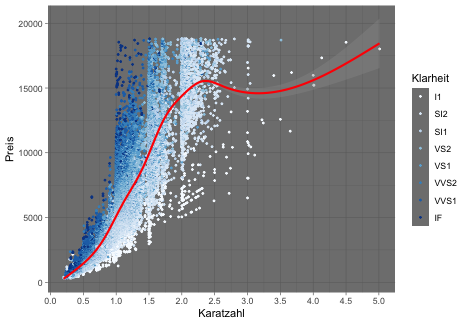
\includegraphics{_main_files/figure-latex/unnamed-chunk-18-1.png}

\hypertarget{aufgaben}{%
\subsection{Aufgaben}\label{aufgaben}}

\begin{enumerate}
\def\labelenumi{\arabic{enumi}.}
\item
  Versuchen Sie, die folgenden Visualisierungen des Datensatzes \texttt{diamonds} auszugeben:

  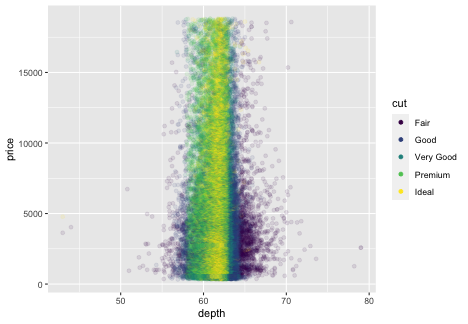
\includegraphics{_main_files/figure-latex/unnamed-chunk-19-1.png}

  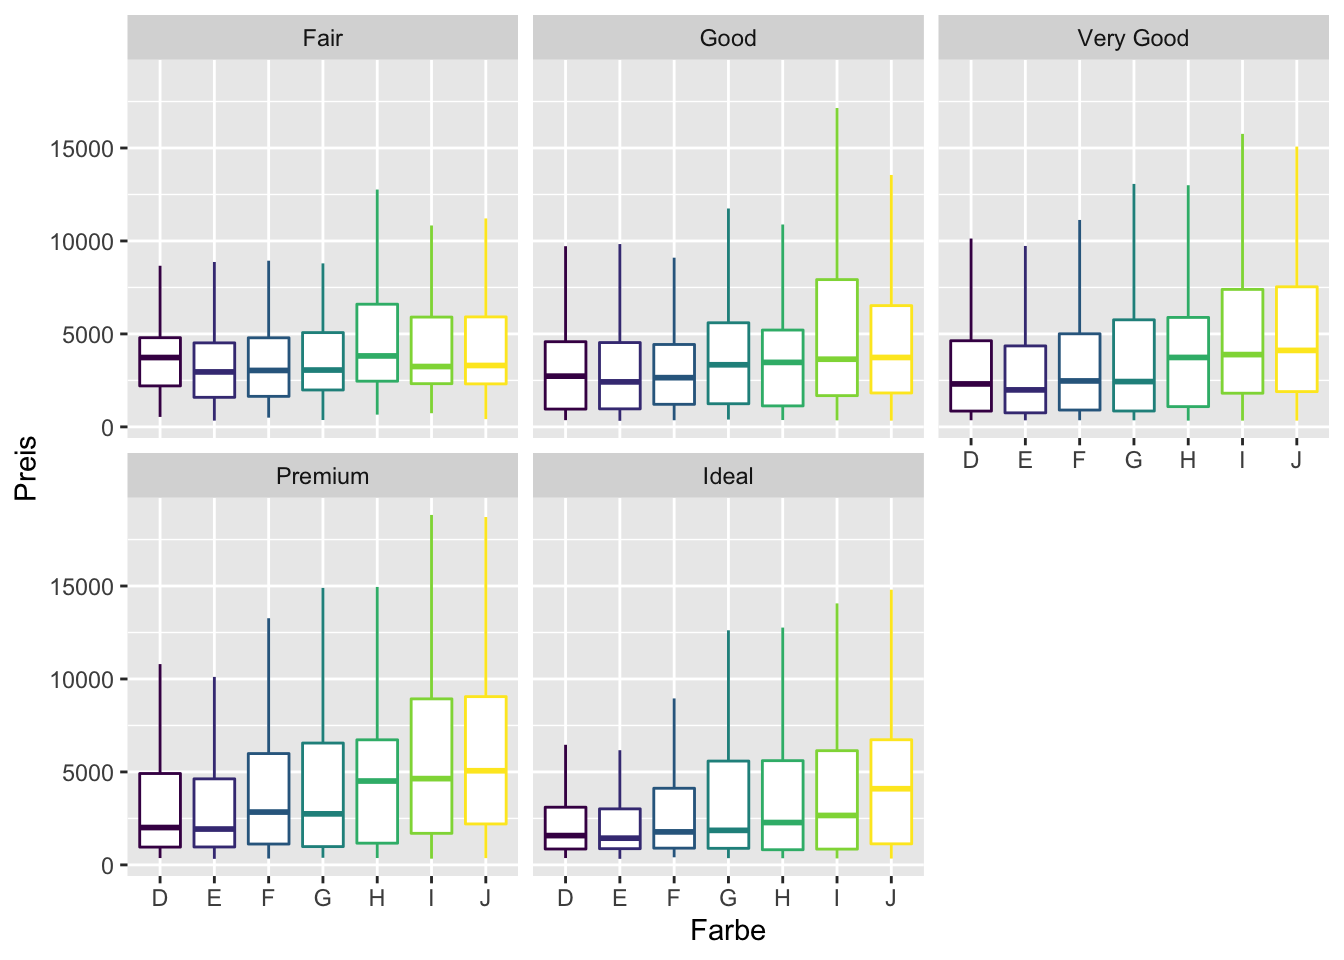
\includegraphics{_main_files/figure-latex/unnamed-chunk-20-1.png}

  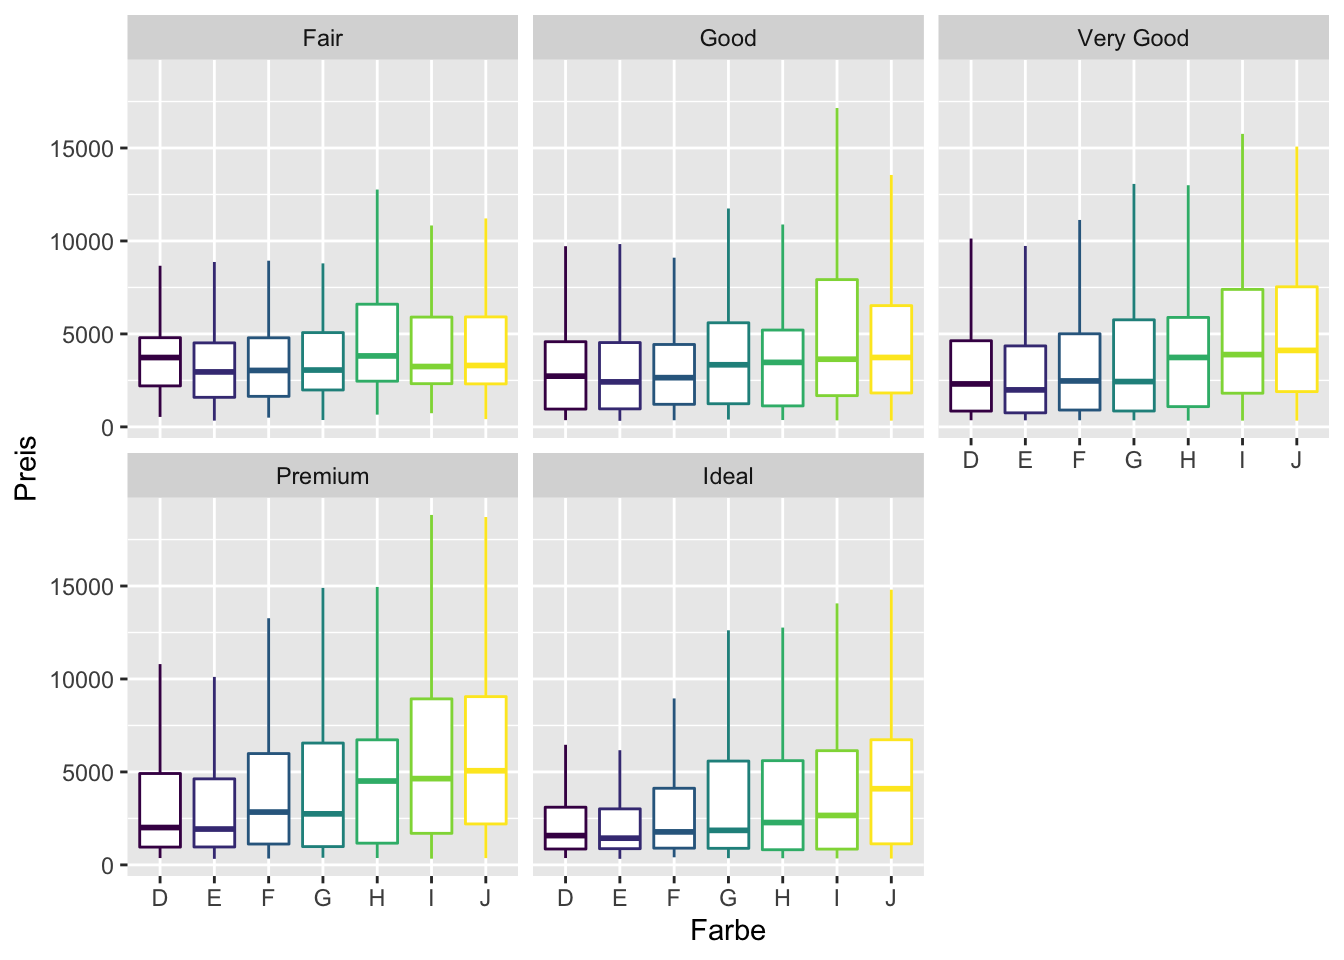
\includegraphics{_main_files/figure-latex/unnamed-chunk-21-1.png}
\item
  Schauen Sie sich die Publikation \href{https://r4ds.had.co.nz/}{R for Data Science} an.
\item
  Was ist das für ein Buch? Wer ist das Zielpublikum?
\item
  Lesen Sie das Kapitel ``3: Data Visualization'' und vollziehen Sie die Visualisierungen nach.
\item
  Bearbeiten Sie die Aufgaben.
\item
  Bearbeiten Sie die \href{https://rstudio.cloud/learn/primers/3}{RStudio Primers zu Datenvisualisierung}.
\end{enumerate}

\hypertarget{karten-erstellen-ftr}{%
\section{Karten erstellen (FTR)}\label{karten-erstellen-ftr}}

\hypertarget{lernziele-dieser-sitzung-1}{%
\subsection{Lernziele dieser Sitzung}\label{lernziele-dieser-sitzung-1}}

Sie können\ldots{}

\begin{itemize}
\tightlist
\item
  Pipes benutzen
\item
  einfache \texttt{dplyr}-Befehle ausführen
\item
  Koordinaten visualisieren
\end{itemize}

\hypertarget{voraussetzungen-1}{%
\subsection{Voraussetzungen}\label{voraussetzungen-1}}

Wir laden erstmal \texttt{tidyverse}:

\begin{Shaded}
\begin{Highlighting}[]
\FunctionTok{library}\NormalTok{(tidyverse)}
\end{Highlighting}
\end{Shaded}

\hypertarget{exkurs-pipes}{%
\subsection{Exkurs: Pipes}\label{exkurs-pipes}}

Teil vom \texttt{tidyverse} ist auch das Paket \texttt{magrittr}, das einen besonderen Operator enthält: \texttt{\%\textgreater{}\%}

Der Operator \texttt{\%\textgreater{}\%} heißt ``Pipe'' und setzt das Ergebnis der vorherigen Funktion als ersten Parameter in die nächste Funktion ein. Zur Veranschaulichung:

\begin{Shaded}
\begin{Highlighting}[]
\NormalTok{anzahl\_buchstaben }\OtherTok{\textless{}{-}} \FunctionTok{length}\NormalTok{(letters)}
\FunctionTok{sqrt}\NormalTok{(anzahl\_buchstaben)}
\end{Highlighting}
\end{Shaded}

\ldots ist das gleiche wie\ldots{}

\begin{Shaded}
\begin{Highlighting}[]
\FunctionTok{sqrt}\NormalTok{(}\FunctionTok{length}\NormalTok{(letters))}
\end{Highlighting}
\end{Shaded}

\ldots ist das gleiche wie\ldots{}

\begin{Shaded}
\begin{Highlighting}[]
\FunctionTok{length}\NormalTok{(letters) }\SpecialCharTok{\%\textgreater{}\%}
  \FunctionTok{sqrt}\NormalTok{()}
\end{Highlighting}
\end{Shaded}

\ldots ist das gleiche wie\ldots{}

\begin{Shaded}
\begin{Highlighting}[]
\NormalTok{letters }\SpecialCharTok{\%\textgreater{}\%}
\NormalTok{  length }\SpecialCharTok{\%\textgreater{}\%}
  \FunctionTok{sqrt}\NormalTok{()}
\end{Highlighting}
\end{Shaded}

So können beliebig viele Funktionen aneinandergereiht werden. Und mit \texttt{-\textgreater{}} kann eine Variable „in die andere Richtung`` zugewiesen werden

\begin{Shaded}
\begin{Highlighting}[]
\NormalTok{letters }\SpecialCharTok{\%\textgreater{}\%}
  \FunctionTok{length}\NormalTok{() }\SpecialCharTok{\%\textgreater{}\%}
  \FunctionTok{sqrt}\NormalTok{() }\SpecialCharTok{\%\textgreater{}\%}
  \FunctionTok{round}\NormalTok{() }\SpecialCharTok{\%\textgreater{}\%}
  \FunctionTok{as.character}\NormalTok{() }\OtherTok{{-}\textgreater{}}
\NormalTok{  my\_var}
\end{Highlighting}
\end{Shaded}

Gerade bei komplizierteren Zusammenhängen wird der Code so oft lesbarer, weil die Logik von links nach rechts, bzw. von oben nach unten gelesen werden kann.

\hypertarget{daten-importieren}{%
\subsection{Daten importieren}\label{daten-importieren}}

Beim Open-Data-Portal der Stadt Frankfurt steht ein \href{http://offenedaten.frankfurt.de/dataset/baumkataster-frankfurt-am-main}{Baumkataster} zur Verfügung.

Die Datei im CSV-Format (comma separated values) kann entweder heruntergeladen und durch klicken importiert werden, oder direkt über den Befehl:

\begin{Shaded}
\begin{Highlighting}[]
\NormalTok{baumkataster }\OtherTok{\textless{}{-}} \FunctionTok{read\_csv2}\NormalTok{(}\StringTok{"http://offenedaten.frankfurt.de/dataset/73c5a6b3{-}c033{-}4dad{-}bb7d{-}8783427dd233/resource/7a73520b{-}961a{-}4aad{-}a582{-}449e676c247c/download/gprojekteopen{-}datadatenamt{-}67datenbaumauswahl\_veroffentlichung\_4baumauswahl\_veroffentlichung\_4.csv"}\NormalTok{)}
\end{Highlighting}
\end{Shaded}

\hypertarget{uxfcberblick-verschaffen}{%
\subsection{Überblick verschaffen}\label{uxfcberblick-verschaffen}}

Mit \texttt{summary()} lässt sich eine Zusammenfassung der Werte generieren:

\begin{Shaded}
\begin{Highlighting}[]
\FunctionTok{summary}\NormalTok{(baumkataster)}
\DocumentationTok{\#\#  Gattung/Art/Deutscher Name   Baumnummer         Objekt            Pflanzjahr  }
\DocumentationTok{\#\#  Length:118403              Min.   :    1.0   Length:118403      Min.   :1645  }
\DocumentationTok{\#\#  Class :character           1st Qu.:   24.0   Class :character   1st Qu.:1970  }
\DocumentationTok{\#\#  Mode  :character           Median :   82.0   Mode  :character   Median :1982  }
\DocumentationTok{\#\#                             Mean   :  232.7                      Mean   :1979  }
\DocumentationTok{\#\#                             3rd Qu.:  270.0                      3rd Qu.:1995  }
\DocumentationTok{\#\#                             Max.   :20158.0                      Max.   :2017  }
\DocumentationTok{\#\#                             NA\textquotesingle{}s   :1853                                       }
\DocumentationTok{\#\#  Kronendurchmesser    HOCHWERT         RECHTSWERT    }
\DocumentationTok{\#\#  Min.   : 2.000    Min.   :5545117   Min.   :463163  }
\DocumentationTok{\#\#  1st Qu.: 4.000    1st Qu.:5550428   1st Qu.:472715  }
\DocumentationTok{\#\#  Median : 6.000    Median :5552601   Median :475219  }
\DocumentationTok{\#\#  Mean   : 6.688    Mean   :5552953   Mean   :475244  }
\DocumentationTok{\#\#  3rd Qu.: 9.000    3rd Qu.:5555165   3rd Qu.:478201  }
\DocumentationTok{\#\#  Max.   :63.000    Max.   :5563639   Max.   :485361  }
\DocumentationTok{\#\# }
\end{Highlighting}
\end{Shaded}

Genauere Infos über diese Merkmale gibt es auf dem Datenportal.

\hypertarget{visualisieren}{%
\subsection{Visualisieren}\label{visualisieren}}

Wie in der letzten Lektion besprochen, lässt sich der Datensatz mit \texttt{ggplot()} visualisieren, z.~B.:

\begin{Shaded}
\begin{Highlighting}[]
\FunctionTok{ggplot}\NormalTok{(baumkataster, }\FunctionTok{aes}\NormalTok{(}\AttributeTok{x =}\NormalTok{ Kronendurchmesser)) }\SpecialCharTok{+}
  \FunctionTok{geom\_histogram}\NormalTok{()}
\end{Highlighting}
\end{Shaded}

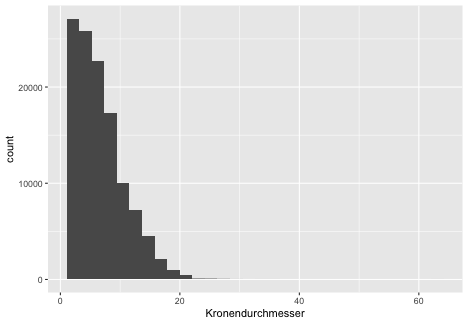
\includegraphics{_main_files/figure-latex/unnamed-chunk-30-1.png}

Eine neue Messreihe lässt sich z.~B. so errechnen:

\begin{Shaded}
\begin{Highlighting}[]
\NormalTok{alter }\OtherTok{\textless{}{-}} \DecValTok{2020} \SpecialCharTok{{-}}\NormalTok{ baumkataster}\SpecialCharTok{$}\NormalTok{Pflanzjahr}
\FunctionTok{head}\NormalTok{(alter)}
\DocumentationTok{\#\# [1] 100 100 100 100 100 100}
\end{Highlighting}
\end{Shaded}

Der Befehl \texttt{mutate()} funktioniert sehr ähnlich, gibt aber den veränderten Datensatz zurück:

\begin{Shaded}
\begin{Highlighting}[]
\FunctionTok{mutate}\NormalTok{(baumkataster, }\AttributeTok{alter =} \DecValTok{2020} \SpecialCharTok{{-}}\NormalTok{ Pflanzjahr)}
\DocumentationTok{\#\# \# A tibble: 118,403 x 8}
\DocumentationTok{\#\#    \textasciigrave{}Gattung/Art/Deutsch\textasciitilde{} Baumnummer Objekt  Pflanzjahr Kronendurchmess\textasciitilde{} HOCHWERT}
\DocumentationTok{\#\#    \textless{}chr\textgreater{}                      \textless{}dbl\textgreater{} \textless{}chr\textgreater{}        \textless{}dbl\textgreater{}            \textless{}dbl\textgreater{}    \textless{}dbl\textgreater{}}
\DocumentationTok{\#\#  1 Platanus x hispanica\textasciitilde{}          1 Ackerm\textasciitilde{}       1920                8 5549511.}
\DocumentationTok{\#\#  2 Platanus x hispanica\textasciitilde{}          2 Ackerm\textasciitilde{}       1920                8 5549517.}
\DocumentationTok{\#\#  3 Platanus x hispanica\textasciitilde{}          3 Ackerm\textasciitilde{}       1920                8 5549524.}
\DocumentationTok{\#\#  4 Platanus x hispanica\textasciitilde{}          4 Ackerm\textasciitilde{}       1920                8 5549531 }
\DocumentationTok{\#\#  5 Platanus x hispanica\textasciitilde{}          5 Ackerm\textasciitilde{}       1920                8 5549538.}
\DocumentationTok{\#\#  6 Platanus x hispanica\textasciitilde{}          6 Ackerm\textasciitilde{}       1920                8 5549544.}
\DocumentationTok{\#\#  7 Platanus x hispanica\textasciitilde{}          7 Ackerm\textasciitilde{}       1920                8 5549551.}
\DocumentationTok{\#\#  8 Platanus x hispanica\textasciitilde{}          8 Ackerm\textasciitilde{}       1920                8 5549557.}
\DocumentationTok{\#\#  9 Platanus x hispanica\textasciitilde{}          9 Ackerm\textasciitilde{}       1920                8 5549564.}
\DocumentationTok{\#\# 10 Platanus x hispanica\textasciitilde{}         10 Ackerm\textasciitilde{}       1920                8 5549571.}
\DocumentationTok{\#\# \# ... with 118,393 more rows, and 2 more variables: RECHTSWERT \textless{}dbl\textgreater{},}
\DocumentationTok{\#\# \#   alter \textless{}dbl\textgreater{}}
\end{Highlighting}
\end{Shaded}

Derselbe Befehl mit dem Pipe-Operator:

\begin{Shaded}
\begin{Highlighting}[]
\NormalTok{baumkataster }\SpecialCharTok{\%\textgreater{}\%}
  \FunctionTok{mutate}\NormalTok{(}\AttributeTok{alter =} \DecValTok{2020} \SpecialCharTok{{-}}\NormalTok{ Pflanzjahr)}
\DocumentationTok{\#\# \# A tibble: 118,403 x 8}
\DocumentationTok{\#\#    \textasciigrave{}Gattung/Art/Deutsch\textasciitilde{} Baumnummer Objekt  Pflanzjahr Kronendurchmess\textasciitilde{} HOCHWERT}
\DocumentationTok{\#\#    \textless{}chr\textgreater{}                      \textless{}dbl\textgreater{} \textless{}chr\textgreater{}        \textless{}dbl\textgreater{}            \textless{}dbl\textgreater{}    \textless{}dbl\textgreater{}}
\DocumentationTok{\#\#  1 Platanus x hispanica\textasciitilde{}          1 Ackerm\textasciitilde{}       1920                8 5549511.}
\DocumentationTok{\#\#  2 Platanus x hispanica\textasciitilde{}          2 Ackerm\textasciitilde{}       1920                8 5549517.}
\DocumentationTok{\#\#  3 Platanus x hispanica\textasciitilde{}          3 Ackerm\textasciitilde{}       1920                8 5549524.}
\DocumentationTok{\#\#  4 Platanus x hispanica\textasciitilde{}          4 Ackerm\textasciitilde{}       1920                8 5549531 }
\DocumentationTok{\#\#  5 Platanus x hispanica\textasciitilde{}          5 Ackerm\textasciitilde{}       1920                8 5549538.}
\DocumentationTok{\#\#  6 Platanus x hispanica\textasciitilde{}          6 Ackerm\textasciitilde{}       1920                8 5549544.}
\DocumentationTok{\#\#  7 Platanus x hispanica\textasciitilde{}          7 Ackerm\textasciitilde{}       1920                8 5549551.}
\DocumentationTok{\#\#  8 Platanus x hispanica\textasciitilde{}          8 Ackerm\textasciitilde{}       1920                8 5549557.}
\DocumentationTok{\#\#  9 Platanus x hispanica\textasciitilde{}          9 Ackerm\textasciitilde{}       1920                8 5549564.}
\DocumentationTok{\#\# 10 Platanus x hispanica\textasciitilde{}         10 Ackerm\textasciitilde{}       1920                8 5549571.}
\DocumentationTok{\#\# \# ... with 118,393 more rows, and 2 more variables: RECHTSWERT \textless{}dbl\textgreater{},}
\DocumentationTok{\#\# \#   alter \textless{}dbl\textgreater{}}
\end{Highlighting}
\end{Shaded}

So lassen sich auch hier verschiedene Befehle verknüpfen. \texttt{filter()} beschränkt den Datensatz auf Merkmalsträger, die den Kriterien entsprechen:

\begin{Shaded}
\begin{Highlighting}[]
\NormalTok{baumkataster }\SpecialCharTok{\%\textgreater{}\%}
  \FunctionTok{mutate}\NormalTok{(}\AttributeTok{alter =} \DecValTok{2020} \SpecialCharTok{{-}}\NormalTok{ Pflanzjahr) }\SpecialCharTok{\%\textgreater{}\%}
  \FunctionTok{filter}\NormalTok{(alter }\SpecialCharTok{\textgreater{}} \DecValTok{30}\NormalTok{) }\OtherTok{{-}\textgreater{}}
\NormalTok{  alte\_baeume}

\FunctionTok{summary}\NormalTok{(alte\_baeume)}
\DocumentationTok{\#\#  Gattung/Art/Deutscher Name   Baumnummer         Objekt            Pflanzjahr  }
\DocumentationTok{\#\#  Length:73859               Min.   :    1.0   Length:73859       Min.   :1645  }
\DocumentationTok{\#\#  Class :character           1st Qu.:   29.0   Class :character   1st Qu.:1960  }
\DocumentationTok{\#\#  Mode  :character           Median :   97.0   Mode  :character   Median :1974  }
\DocumentationTok{\#\#                             Mean   :  263.2                      Mean   :1966  }
\DocumentationTok{\#\#                             3rd Qu.:  314.0                      3rd Qu.:1980  }
\DocumentationTok{\#\#                             Max.   :10489.0                      Max.   :1989  }
\DocumentationTok{\#\#                             NA\textquotesingle{}s   :684                                        }
\DocumentationTok{\#\#  Kronendurchmesser    HOCHWERT         RECHTSWERT         alter       }
\DocumentationTok{\#\#  Min.   : 2.000    Min.   :5545117   Min.   :463163   Min.   : 31.00  }
\DocumentationTok{\#\#  1st Qu.: 6.000    1st Qu.:5550415   1st Qu.:472667   1st Qu.: 40.00  }
\DocumentationTok{\#\#  Median : 8.000    Median :5552480   Median :475708   Median : 46.00  }
\DocumentationTok{\#\#  Mean   : 8.503    Mean   :5552593   Mean   :475402   Mean   : 53.54  }
\DocumentationTok{\#\#  3rd Qu.:10.000    3rd Qu.:5554589   3rd Qu.:478539   3rd Qu.: 60.00  }
\DocumentationTok{\#\#  Max.   :35.000    Max.   :5563639   Max.   :485360   Max.   :375.00  }
\DocumentationTok{\#\# }
\end{Highlighting}
\end{Shaded}

Schließlich ergibt das Streudiagramm von Koordinaten so eine art Karte:

\begin{Shaded}
\begin{Highlighting}[]
\FunctionTok{ggplot}\NormalTok{(alte\_baeume) }\SpecialCharTok{+}
    \FunctionTok{geom\_point}\NormalTok{(}\AttributeTok{size =} \FloatTok{0.1}\NormalTok{, }\FunctionTok{aes}\NormalTok{(}\AttributeTok{x =}\NormalTok{ RECHTSWERT, }\AttributeTok{y =}\NormalTok{ HOCHWERT))}
\end{Highlighting}
\end{Shaded}

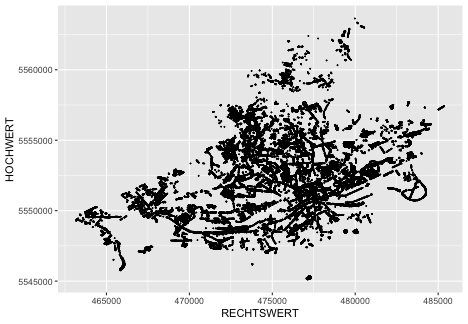
\includegraphics{_main_files/figure-latex/unnamed-chunk-35-1.png}

Diesen Ansatz werden wir in der nächsten Lektion vertiefen.

\hypertarget{karten-erstellen-hos}{%
\section{Karten erstellen (HOS)}\label{karten-erstellen-hos}}

\hypertarget{aufgaben-1}{%
\subsection{Aufgaben}\label{aufgaben-1}}

\begin{enumerate}
\def\labelenumi{\arabic{enumi}.}
\item
  Besuchen Sie \url{https://pleiades.stoa.org/} - worum geht es hier?
\item
  Finden Sie den kompletten aktuellen Datensatz für „locations`` als CSV-Datei.
\item
  Importieren Sie ihn in R und weisen Sie dem Datensatz den Namen \texttt{pleiades} zu.
\item
  Finden Sie geeignete Werte für (einzelne) Längen- und Breitengrade im Datensatz.
\item
  Plotten Sie die Koordinaten auf x- und y-Achse mit \texttt{ggplot()}. Was erkennen Sie?
\item
  Halbieren Sie die Größe und setzen Sie den Alpha-Wert der Punkte auf 0,2.
\item
  Bringen Sie die Grafik in die Mercator-Projektion.
\item
  Schauen Sie sich diesen Befehl an:

\begin{Shaded}
\begin{Highlighting}[]
\FunctionTok{map\_data}\NormalTok{(}\StringTok{"world"}\NormalTok{) }\SpecialCharTok{\%\textgreater{}\%}
  \FunctionTok{ggplot}\NormalTok{() }\SpecialCharTok{+}
    \FunctionTok{geom\_polygon}\NormalTok{(}\AttributeTok{mapping =} \FunctionTok{aes}\NormalTok{(}\AttributeTok{x =}\NormalTok{ long,}
                               \AttributeTok{y =}\NormalTok{ lat,}
                               \AttributeTok{group =}\NormalTok{ group)) }\SpecialCharTok{+}
    \FunctionTok{coord\_quickmap}\NormalTok{(}\AttributeTok{xlim =} \FunctionTok{c}\NormalTok{(}\SpecialCharTok{{-}}\DecValTok{8}\NormalTok{, }\DecValTok{40}\NormalTok{),}
                   \AttributeTok{ylim =} \FunctionTok{c}\NormalTok{(}\DecValTok{26}\NormalTok{, }\DecValTok{48}\NormalTok{))}
\end{Highlighting}
\end{Shaded}
\item
  Versuchen Sie, jede einzelne Zeile nachzuvollziehen, indem Sie die entsprechenden Funktionen recherchieren.
\item
  Führen Sie den Befehl aus.
\item
  Ändern Sie die Farbe der Flächen in hellgrau.
\item
  Wählen Sie einen Kartenausschnitt, auf dem Portugal, Ägypten, Irak und Frankreich komplett zu sehen sind.
\item
  Plotten Sie auf diesem Hintergrund den Datensatz \texttt{pleiades}. Passen Sie dabei die Parameter so an, dass es Ihnen optisch zusagt.
\item
  Wählen Sie für die Karte die \href{https://de.wikipedia.org/wiki/Bonnesche_Projektion}{Bonnesche Projektion} mit Standardparallele bei 40°N.
\item
  Entfernen Sie alle Achsenbeschriftungen.
\item
  (Achtung: knifflig!) Bilden Sie diese Grafik nach, die die Orte geordnet nach ältestem Fund darstellt:

  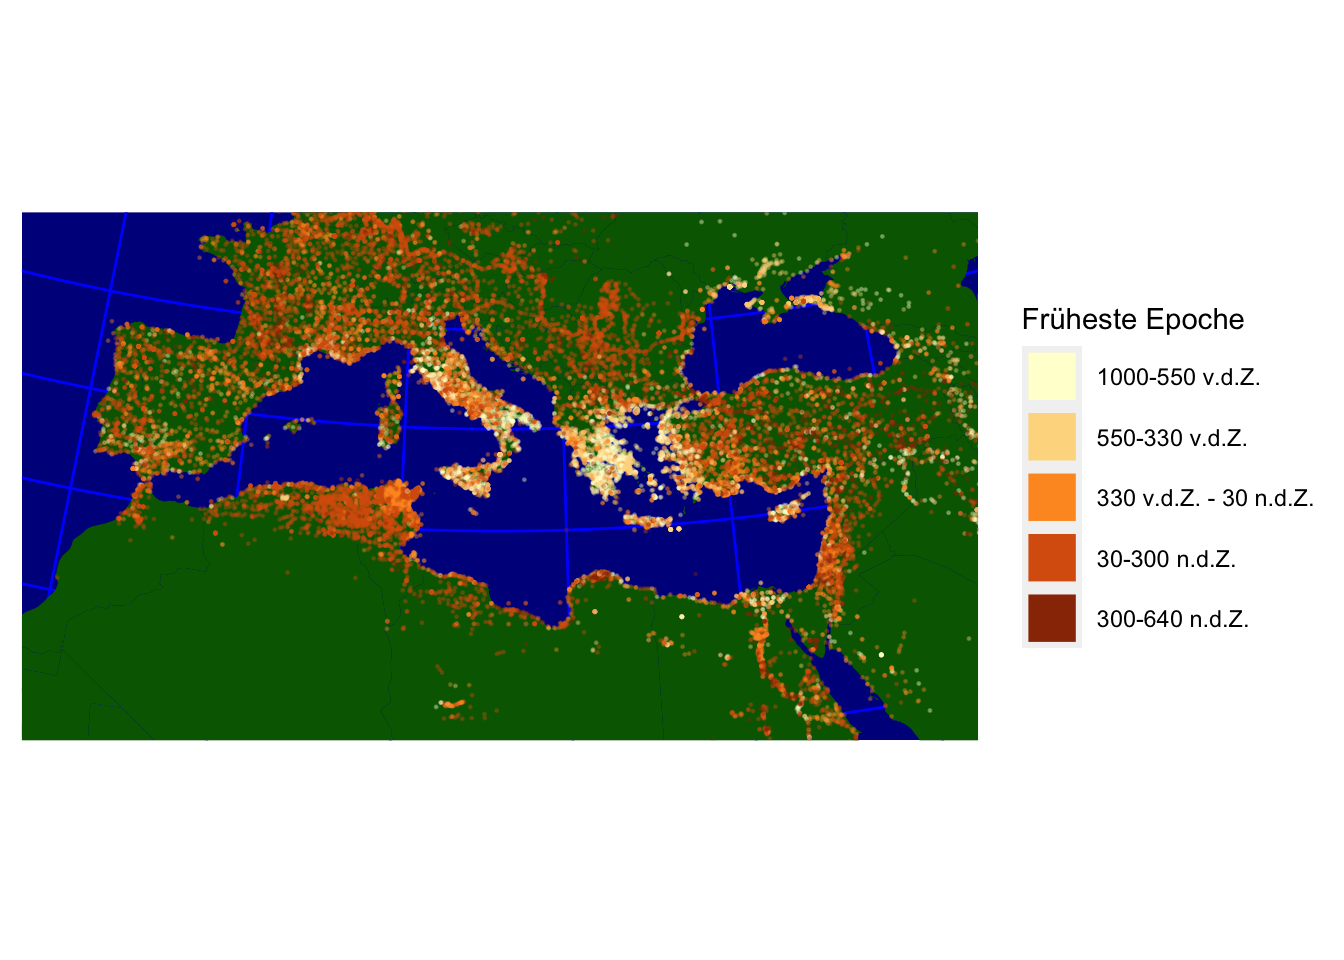
\includegraphics{_main_files/figure-latex/unnamed-chunk-49-1.png}
\end{enumerate}

\hypertarget{geodaten-beschaffen}{%
\section{Geodaten beschaffen}\label{geodaten-beschaffen}}

\hypertarget{lernziele-dieser-sitzung-2}{%
\subsection{Lernziele dieser Sitzung}\label{lernziele-dieser-sitzung-2}}

Sie können\ldots{}

\begin{itemize}
\tightlist
\item
  sich den Quellcode einer Webseite anzeigen lassen und interpretieren.
\item
  HTML-Tabellen als Datensatz einlesen.
\item
  Fortgeschrittene Methoden der Datenbereinigung nachvollziehen.
\end{itemize}

\hypertarget{vorbereitung}{%
\subsection{Vorbereitung}\label{vorbereitung}}

Am Beispiel der Küstenlängen verschiedener Länder besprechen wir Techniken der Datenerhebung/-erfassung und -visualisierung. Unser Ziel ist es, die Daten zu den Küstenlängen in einer Grafik darzustellen.

Für die folgenden Aufgaben benötigen wir die Pakete \texttt{rvest} und \texttt{tidyverse}. Zunächst müssen diese installiert und in unsere Umgebung geladen werden.

\begin{Shaded}
\begin{Highlighting}[]
\FunctionTok{library}\NormalTok{(tidyverse)}
\FunctionTok{library}\NormalTok{(rvest)}
\end{Highlighting}
\end{Shaded}

\hypertarget{datenbeschaffung}{%
\subsection{Datenbeschaffung}\label{datenbeschaffung}}

Auf dem Internetauftritt der CIA gab es es eine Tabelle, welche die Küstenlänge (inklusive der Inseln) der einzelnen Länder enthält.

Über die Archivierungsplattform WayBackMachine ist die Seite immer noch abrufbar: \url{https://web.archive.org/web/20190802010710/https://www.cia.gov/library/publications/the-world-factbook/fields/282.html}

In einem ersten Schritt wird die URL der Tabelle der Variable \texttt{url} zugewiesen, sodass der Quellcode mit dem Befehl \texttt{read\_html()} eingelesen werden kann.

\begin{Shaded}
\begin{Highlighting}[]
\NormalTok{url }\OtherTok{\textless{}{-}} \StringTok{"https://web.archive.org/web/20190802010710/https://www.cia.gov/library/publications/the{-}world{-}factbook/fields/282.html"}
\NormalTok{reply }\OtherTok{\textless{}{-}} \FunctionTok{read\_html}\NormalTok{(url)}
\end{Highlighting}
\end{Shaded}

Der Befehl \texttt{html\_table()} ermöglicht das Auslesen \emph{aller} Tabellen auf der Seite. Mithilfe des Befehls \texttt{str()} sehen wir, dass die Seite genau eine Tabelle enthält, welche die Informationen zu den Küstenlängen enthält.

\begin{Shaded}
\begin{Highlighting}[]
\NormalTok{tables }\OtherTok{\textless{}{-}} \FunctionTok{html\_table}\NormalTok{(reply, }\AttributeTok{fill =} \ConstantTok{TRUE}\NormalTok{)}
\FunctionTok{str}\NormalTok{(tables)}
\DocumentationTok{\#\# List of 1}
\DocumentationTok{\#\#  $ : tibble [266 x 2] (S3: tbl\_df/tbl/data.frame)}
\DocumentationTok{\#\#   ..$ Country  : chr [1:266] "Afghanistan" "Akrotiri" "Albania" "Algeria" ...}
\DocumentationTok{\#\#   ..$ Coastline: chr [1:266] "0 km\textbackslash{}n          (landlocked)" "56.3 km" "362 km" "998 km" ...}
\end{Highlighting}
\end{Shaded}

Durch die Umformung zu einem tibble erhalten wir eine Tabelle mit den gewünschten Informationen:

\begin{Shaded}
\begin{Highlighting}[]
\FunctionTok{as\_tibble}\NormalTok{(tables[[}\DecValTok{1}\NormalTok{]])}
\DocumentationTok{\#\# \# A tibble: 266 x 2}
\DocumentationTok{\#\#    Country             Coastline                     }
\DocumentationTok{\#\#    \textless{}chr\textgreater{}               \textless{}chr\textgreater{}                         }
\DocumentationTok{\#\#  1 Afghanistan         "0 km\textbackslash{}n          (landlocked)"}
\DocumentationTok{\#\#  2 Akrotiri            "56.3 km"                     }
\DocumentationTok{\#\#  3 Albania             "362 km"                      }
\DocumentationTok{\#\#  4 Algeria             "998 km"                      }
\DocumentationTok{\#\#  5 American Samoa      "116 km"                      }
\DocumentationTok{\#\#  6 Andorra             "0 km\textbackslash{}n          (landlocked)"}
\DocumentationTok{\#\#  7 Angola              "1,600 km"                    }
\DocumentationTok{\#\#  8 Anguilla            "61 km"                       }
\DocumentationTok{\#\#  9 Antarctica          "17,968 km"                   }
\DocumentationTok{\#\# 10 Antigua and Barbuda "153 km"                      }
\DocumentationTok{\#\# \# ... with 256 more rows}
\end{Highlighting}
\end{Shaded}

Mit pipes können wir die obigen Befehle zusammenfassen und somit das Ganze auf einmal ausführen.

\begin{Shaded}
\begin{Highlighting}[]
\StringTok{"https://web.archive.org/web/20190802010710/https://www.cia.gov/library/publications/the{-}world{-}factbook/fields/282.html"} \SpecialCharTok{\%\textgreater{}\%}
  \FunctionTok{read\_html}\NormalTok{() }\SpecialCharTok{\%\textgreater{}\%}
  \FunctionTok{html\_table}\NormalTok{(}\AttributeTok{fill =}\NormalTok{ T) }\SpecialCharTok{\%\textgreater{}\%}
\NormalTok{  .[[}\DecValTok{1}\NormalTok{]] }\SpecialCharTok{\%\textgreater{}\%}
  \FunctionTok{as\_tibble}\NormalTok{() }\OtherTok{{-}\textgreater{}}\NormalTok{ coast}
\end{Highlighting}
\end{Shaded}

\hypertarget{datenformatierung}{%
\subsection{Datenformatierung}\label{datenformatierung}}

Zur Datenformatierung nutzen wir Funktionen aus dem Paket \texttt{stringr}. Die Spalte mit der Küstenlänge soll keinen Text, keine Einheit direkt hinter den Zahlenwerten und keine Kommata zur Trennung der Zahlenwerte enthalten.

Der Befehl ``str\_extract()'' sucht nach vorgegebenen Mustern (engl. \emph{patterns}) und wählt diese aus. Diese patterns werden auch reguläre Ausdrücke (\emph{regular expressions / regex}) genannt und sind eigentlich \href{https://danielfett.de/en/tutorials/tutorial-regulare-ausdrucke/}{ein Thema für sich}. Das Pattern \texttt{{[}0-9,.{]}+\ km} extrahiert die Kilometerangaben.

\begin{Shaded}
\begin{Highlighting}[]
\NormalTok{km }\OtherTok{\textless{}{-}} \FunctionTok{str\_extract}\NormalTok{(coast}\SpecialCharTok{$}\NormalTok{Coastline, }\StringTok{"[0{-}9,.]+ km"}\NormalTok{)}
\end{Highlighting}
\end{Shaded}

Die ausgewählten Muster (in unserem Fall Kommata und Text) können durch den Befehl \texttt{str\_replace\_all()} gelöscht oder ersetzt werden. Wir ersetzen alle Zeichen \emph{außer} Zahlen und Dezimalpunkt mit einem leeren String, so dass sie verschwinden.

\begin{Shaded}
\begin{Highlighting}[]
\FunctionTok{str\_replace\_all}\NormalTok{(km, }\StringTok{"[\^{}0{-}9.]"}\NormalTok{, }\StringTok{""}\NormalTok{)}
\DocumentationTok{\#\#   [1] "0"       "56.3"    "362"     "998"     "116"     "0"       "1600"   }
\DocumentationTok{\#\#   [8] "61"      "17968"   "153"     "45389"   "4989"    "0"       "68.5"   }
\DocumentationTok{\#\#  [15] "74.1"    "111866"  "25760"   "0"       "0"       "3542"    "161"    }
\DocumentationTok{\#\#  [22] "580"     "97"      "0"       "66.5"    "386"     "121"     "103"    }
\DocumentationTok{\#\#  [29] "0"       "0"       "20"      "0"       "29.6"    "7491"    "698"    }
\DocumentationTok{\#\#  [36] "80"      "161"     "354"     "0"       "1930"    "0"       "965"    }
\DocumentationTok{\#\#  [43] "443"     "402"     "202080"  "160"     "0"       "0"       "6435"   }
\DocumentationTok{\#\#  [50] "14500"   "138.9"   "11.1"    "26"      "3208"    "340"     "37"     }
\DocumentationTok{\#\#  [57] "169"     "120"     "3095"    "1290"    "515"     "5835"    "3735"   }
\DocumentationTok{\#\#  [64] "364"     "648"     "0"       "7314"    "27.5"    "314"     "148"    }
\DocumentationTok{\#\#  [71] "1288"    "2237"    "2450"    "307"     "296"     "2234"    "3794"   }
\DocumentationTok{\#\#  [78] "0"       "0"       "65992.9" "1288"    "1117"    "1129"    "1250"   }
\DocumentationTok{\#\#  [85] "4853"    "2525"    "28"      "885"     "80"      "40"      "310"    }
\DocumentationTok{\#\#  [92] "2389"    "539"     "12"      "13676"   "44087"   "121"     "125.5"  }
\DocumentationTok{\#\#  [99] "400"     "50"      "320"     "350"     "459"     "1771"    "101.9"  }
\DocumentationTok{\#\# [106] "0"       "823"     "733"     "6.4"     "0"       "4970"    "7000"   }
\DocumentationTok{\#\# [113] "66526"   "54716"   "2440"    "58"      "1448"    "160"     "273"    }
\DocumentationTok{\#\# [120] "7600"    "1022"    "124.1"   "29751"   "8"       "70"      "34"     }
\DocumentationTok{\#\# [127] "26"      "0"       "536"     "3"       "1143"    "2495"    "2413"   }
\DocumentationTok{\#\# [134] "0"       "499"     "0"       "0"       "498"     "225"     "0"      }
\DocumentationTok{\#\# [141] "579"     "1770"    "0"       "90"      "0"       "41"      "4828"   }
\DocumentationTok{\#\# [148] "0"       "4675"    "644"     "0"       "196.8"   "370.4"   "754"    }
\DocumentationTok{\#\# [155] "177"     "9330"    "6112"    "15"      "0"       "4.1"     "0"      }
\DocumentationTok{\#\# [162] "293.5"   "40"      "1835"    "2470"    "1572"    "30"      "8"      }
\DocumentationTok{\#\# [169] "0"       "451"     "2254"    "15134"   "910"     "0"       "853"    }
\DocumentationTok{\#\# [176] "64"      "32"      "0"       "1482"    "25148"   "2092"    "135663" }
\DocumentationTok{\#\# [183] "1046"    "1519"    "14.5"    "2490"    "5152"    "518"     "0"      }
\DocumentationTok{\#\# [190] "2414"    "36289"   "51"      "440"     "1793"    "501"     "563"    }
\DocumentationTok{\#\# [197] "225"     "37653"   "0"       "60"      "135"     "158"     "58.9"   }
\DocumentationTok{\#\# [204] "120"     "84"      "403"     "0"       "209"     "2640"    "531"    }
\DocumentationTok{\#\# [211] "0"       "491"     "402"     "193"     "58.9"    "0"       "46.6"   }
\DocumentationTok{\#\# [218] "5313"    "3025"    "2798"    NA        "0"       "17968"   "4964"   }
\DocumentationTok{\#\# [225] "926"     "1340"    "853"     "386"     "3587"    "3218"    "0"      }
\DocumentationTok{\#\# [232] "193"     "1566.3"  "0"       "1424"    "3219"    "706"     "56"     }
\DocumentationTok{\#\# [239] "101"     "419"     "362"     "1148"    "7200"    "0"       "389"    }
\DocumentationTok{\#\# [246] "24"      "0"       "2782"    "1318"    "12429"   "19924"   "4.8"    }
\DocumentationTok{\#\# [253] "660"     "0"       "2528"    "2800"    "3444"    "188"     "19.3"   }
\DocumentationTok{\#\# [260] "129"     "0"       "1110"    "356000"  "1906"    "0"       "0"}
\end{Highlighting}
\end{Shaded}

Auch hier kann alles in einen Befehl gepackt werden:

\begin{Shaded}
\begin{Highlighting}[]
\NormalTok{coast}\SpecialCharTok{$}\NormalTok{Coastline }\SpecialCharTok{\%\textgreater{}\%}
  \FunctionTok{str\_extract}\NormalTok{(}\StringTok{"[0{-}9,.]+ km"}\NormalTok{) }\SpecialCharTok{\%\textgreater{}\%}
  \FunctionTok{str\_replace\_all}\NormalTok{(}\StringTok{"[\^{}0{-}9.]"}\NormalTok{, }\StringTok{""}\NormalTok{) }\SpecialCharTok{\%\textgreater{}\%}
  \FunctionTok{as.numeric}\NormalTok{() }\OtherTok{{-}\textgreater{}}\NormalTok{ coast}\SpecialCharTok{$}\NormalTok{coast\_num}
\end{Highlighting}
\end{Shaded}

\hypertarget{datenaufbereitung}{%
\subsection{Datenaufbereitung}\label{datenaufbereitung}}

Mit dem Befehl \texttt{arrange()} kann die Tabelle sortiert werden. Zunächst auftseigend,

\begin{Shaded}
\begin{Highlighting}[]
\NormalTok{coast }\SpecialCharTok{\%\textgreater{}\%}
  \FunctionTok{arrange}\NormalTok{(coast\_num)}
\DocumentationTok{\#\# \# A tibble: 266 x 3}
\DocumentationTok{\#\#    Country     Coastline                                               coast\_num}
\DocumentationTok{\#\#    \textless{}chr\textgreater{}       \textless{}chr\textgreater{}                                                       \textless{}dbl\textgreater{}}
\DocumentationTok{\#\#  1 Afghanistan "0 km\textbackslash{}n          (landlocked)"                                  0}
\DocumentationTok{\#\#  2 Andorra     "0 km\textbackslash{}n          (landlocked)"                                  0}
\DocumentationTok{\#\#  3 Armenia     "0 km\textbackslash{}n          (landlocked)"                                  0}
\DocumentationTok{\#\#  4 Austria     "0 km\textbackslash{}n          (landlocked)"                                  0}
\DocumentationTok{\#\#  5 Azerbaijan  "0 km\textbackslash{}n          (landlocked); note {-} Azerbaijan borde\textasciitilde{}         0}
\DocumentationTok{\#\#  6 Belarus     "0 km\textbackslash{}n          (landlocked)"                                  0}
\DocumentationTok{\#\#  7 Bhutan      "0 km\textbackslash{}n          (landlocked)"                                  0}
\DocumentationTok{\#\#  8 Bolivia     "0 km\textbackslash{}n          (landlocked)"                                  0}
\DocumentationTok{\#\#  9 Botswana    "0 km\textbackslash{}n          (landlocked)"                                  0}
\DocumentationTok{\#\# 10 Burkina Fa\textasciitilde{} "0 km\textbackslash{}n          (landlocked)"                                  0}
\DocumentationTok{\#\# \# ... with 256 more rows}
\end{Highlighting}
\end{Shaded}

und schließlich absteigend, sodass die größten Werte an erster Stelle stehen.

\begin{Shaded}
\begin{Highlighting}[]
\NormalTok{coast }\SpecialCharTok{\%\textgreater{}\%}
  \FunctionTok{arrange}\NormalTok{(}\FunctionTok{desc}\NormalTok{(coast\_num))}
\DocumentationTok{\#\# \# A tibble: 266 x 3}
\DocumentationTok{\#\#    Country      Coastline                                              coast\_num}
\DocumentationTok{\#\#    \textless{}chr\textgreater{}        \textless{}chr\textgreater{}                                                      \textless{}dbl\textgreater{}}
\DocumentationTok{\#\#  1 World        "356,000 km\textbackslash{}n          \textbackslash{}n          \textbackslash{}n        \textbackslash{}n\textbackslash{}n  \textbackslash{}n\textasciitilde{}   356000 }
\DocumentationTok{\#\#  2 Canada       "202,080 km\textbackslash{}n          \textbackslash{}n          \textbackslash{}n        \textbackslash{}n\textbackslash{}n  \textbackslash{}n\textasciitilde{}   202080 }
\DocumentationTok{\#\#  3 Pacific Oce\textasciitilde{} "135,663 km"                                             135663 }
\DocumentationTok{\#\#  4 Atlantic Oc\textasciitilde{} "111,866 km"                                             111866 }
\DocumentationTok{\#\#  5 Indian Ocean "66,526 km"                                               66526 }
\DocumentationTok{\#\#  6 European Un\textasciitilde{} "65,992.9 km"                                             65993.}
\DocumentationTok{\#\#  7 Indonesia    "54,716 km"                                               54716 }
\DocumentationTok{\#\#  8 Arctic Ocean "45,389 km"                                               45389 }
\DocumentationTok{\#\#  9 Greenland    "44,087 km"                                               44087 }
\DocumentationTok{\#\# 10 Russia       "37,653 km"                                               37653 }
\DocumentationTok{\#\# \# ... with 256 more rows}
\end{Highlighting}
\end{Shaded}

Bevor wir jedoch eine vollständig sortierte Liste haben, muss der Datensatz noch von falschen Einträgen gesäubert werden. Dafür benutzen wir den Befehl \texttt{filter()}. Wir suchen wieder nach einem bestimmten Muster (hier zum Beispiel dem Wort ``Ocean'') und filtern es aus dem Datensatz.

Die Grafik soll nur aus den ersten 30 Einträgen der Tabelle bestehen, welche uns der Befehl \texttt{head()} ausgibt.

\begin{Shaded}
\begin{Highlighting}[]
\NormalTok{coast }\SpecialCharTok{\%\textgreater{}\%}
  \FunctionTok{arrange}\NormalTok{(}\FunctionTok{desc}\NormalTok{(coast\_num)) }\SpecialCharTok{\%\textgreater{}\%}
  \FunctionTok{filter}\NormalTok{(}\SpecialCharTok{!}\FunctionTok{str\_detect}\NormalTok{(Country, }\StringTok{"Ocean"}\NormalTok{)) }\SpecialCharTok{\%\textgreater{}\%}
  \FunctionTok{filter}\NormalTok{(}\SpecialCharTok{!}\NormalTok{Country }\SpecialCharTok{\%in\%} \FunctionTok{c}\NormalTok{(}\StringTok{"World"}\NormalTok{, }\StringTok{"European Union"}\NormalTok{)) }\SpecialCharTok{\%\textgreater{}\%}
  \FunctionTok{head}\NormalTok{(}\DecValTok{30}\NormalTok{) }\OtherTok{{-}\textgreater{}}\NormalTok{ top\_30}
\end{Highlighting}
\end{Shaded}

\hypertarget{datenvisualisierung}{%
\subsection{Datenvisualisierung}\label{datenvisualisierung}}

Das Balkendiagramm erhalten wir durch den ``ggplot'' Befehl. Hierbei gibt es verschiedenste Einstellmöglichkeiten. Wichitg sind vor allem die Angabe des verwendeten Datensatzes und die Art der Grafik (ob Kartendarstellung oder Balkendiagramm). Desweiteren kann man noch Farben der Eigenschaften, eine Achsenbeschriftung u. v. m. bestimmen.

\begin{Shaded}
\begin{Highlighting}[]
\FunctionTok{ggplot}\NormalTok{(top\_30, }\FunctionTok{aes}\NormalTok{(}\AttributeTok{x =} \FunctionTok{reorder}\NormalTok{(Country, coast\_num), }\AttributeTok{y=}\NormalTok{coast\_num)) }\SpecialCharTok{+}
  \FunctionTok{geom\_bar}\NormalTok{(}\AttributeTok{stat=}\StringTok{\textquotesingle{}identity\textquotesingle{}}\NormalTok{, }\AttributeTok{fill=}\StringTok{"darkblue"}\NormalTok{) }\SpecialCharTok{+}
  \FunctionTok{coord\_flip}\NormalTok{() }\SpecialCharTok{+}
  \FunctionTok{scale\_x\_discrete}\NormalTok{(}\ConstantTok{NULL}\NormalTok{) }\SpecialCharTok{+}
  \FunctionTok{scale\_y\_continuous}\NormalTok{(}\StringTok{"Küstenlinie (km)"}\NormalTok{)}
\end{Highlighting}
\end{Shaded}

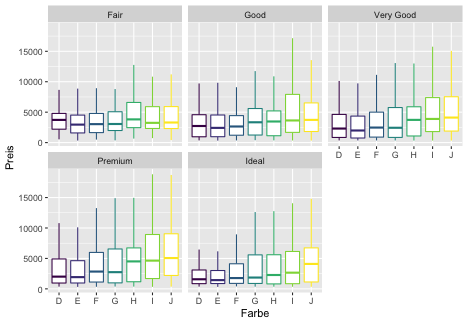
\includegraphics{_main_files/figure-latex/unnamed-chunk-61-1.png}

\hypertarget{aufgaben-2}{%
\subsection{Aufgaben}\label{aufgaben-2}}

\begin{enumerate}
\def\labelenumi{\arabic{enumi}.}
\item
  Importieren Sie die Daten zu den \href{https://en.wikipedia.org/wiki/List_of_deadly_earthquakes_since_1900}{tödlichen Erdbeben auf Wikipedia}
  und formen sie diese zu einem tibble um.
\item
  Erstellen Sie mit den erhaltenen Daten eine Karte, welche die Lage und die Stärke der Erdbeben angibt:

  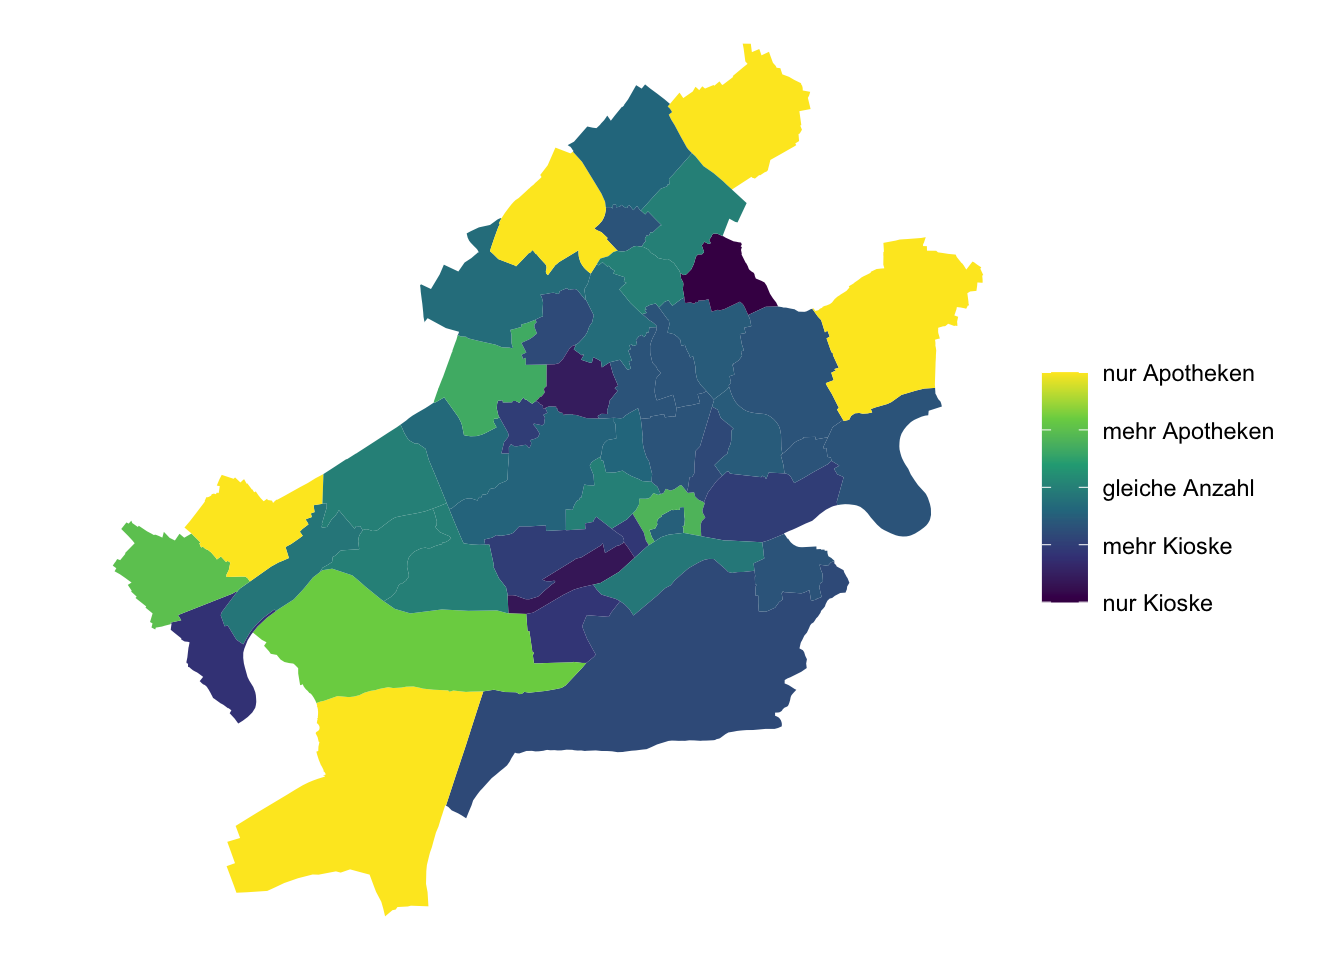
\includegraphics{_main_files/figure-latex/unnamed-chunk-64-1.png}
\item
  Wandeln Sie den Erdbeben-Datensatz in das Simple Features Format um. Laden Sie zusätzlich eine Weltkarte mit dem Paket \texttt{rnaturalearth} und wandeln Sie auch diese in Simple Features um. Finden Sie außerdem einen Geodatensatz zu tektonischen Platten. Visualiseren Sie alles auf einer Welktarte (Projektion: Gall-Peters).
\end{enumerate}

\hypertarget{geodaten-verschneiden}{%
\section{Geodaten verschneiden}\label{geodaten-verschneiden}}

\hypertarget{lernziele}{%
\subsection{Lernziele}\label{lernziele}}

Sie können\ldots{}

\begin{itemize}
\tightlist
\item
  Geodaten als Simple Features importieren,
\item
  CRS bestimmen und umwandeln,
\item
  einfache Verschneidungen von Simple Features durchführen und
\item
  Simple Features kartographisch darstellen.
\end{itemize}

\hypertarget{vorbereitung-1}{%
\subsection{Vorbereitung}\label{vorbereitung-1}}

Für diese Lektion werden zwei Pakete geladen:

\begin{Shaded}
\begin{Highlighting}[]
\FunctionTok{library}\NormalTok{(tidyverse)}
\FunctionTok{library}\NormalTok{(sf)}
\end{Highlighting}
\end{Shaded}

\hypertarget{ziel}{%
\subsection{Ziel}\label{ziel}}

Ziel ist, eine \href{https://de.wikipedia.org/wiki/Choroplethenkarte}{Choroplethenkarte} von Frankfurt zu erstellen, die die Versorgung mit Kiosken darstellt.

\hypertarget{grundkarte}{%
\subsection{Grundkarte}\label{grundkarte}}

Eine Shapefile der Frankfurter Stadtteile findet sich hier: \url{http://www.offenedaten.frankfurt.de/dataset/frankfurter-stadtteilgrenzen-fur-gis-systeme}

Wir laden die Zip-Datei herunter und speichern den enthaltenen Ordner \texttt{stadtteile} in unserem Arbeitsverzeichnis. Es ist eine gute Angewohnheit, einen Unterordner für Ressourcen anzulegen.

Dann importieren wir den Geodatensatz als Simple Features (Paket \texttt{sf}):

\begin{Shaded}
\begin{Highlighting}[]
\NormalTok{stadtteile }\OtherTok{\textless{}{-}} \FunctionTok{st\_read}\NormalTok{(}\StringTok{"resources/stadtteile/Stadtteile\_Frankfurt\_am\_Main.shp"}\NormalTok{)}
\DocumentationTok{\#\# Reading layer \textasciigrave{}Stadtteile\_Frankfurt\_am\_Main\textquotesingle{} from data source }
\DocumentationTok{\#\#   \textasciigrave{}/Users/till/mzs/2021\_methodenwoche/skript/resources/stadtteile/Stadtteile\_Frankfurt\_am\_Main.shp\textquotesingle{} }
\DocumentationTok{\#\#   using driver \textasciigrave{}ESRI Shapefile\textquotesingle{}}
\DocumentationTok{\#\# Simple feature collection with 46 features and 2 fields}
\DocumentationTok{\#\# Geometry type: POLYGON}
\DocumentationTok{\#\# Dimension:     XY}
\DocumentationTok{\#\# Bounding box:  xmin: 462292.7 ymin: 5540412 xmax: 485744.8 ymax: 5563925}
\DocumentationTok{\#\# Projected CRS: ETRS89 / UTM zone 32N}
\end{Highlighting}
\end{Shaded}

Simple Features sind Datensätze, die eine Spalte \texttt{geometry} enthalten, in der Geodaten in einem standardisierten Format hinterlegt sind.

\begin{Shaded}
\begin{Highlighting}[]
\FunctionTok{str}\NormalTok{(stadtteile)}
\DocumentationTok{\#\# Classes \textquotesingle{}sf\textquotesingle{} and \textquotesingle{}data.frame\textquotesingle{}:   46 obs. of  3 variables:}
\DocumentationTok{\#\#  $ STTLNR  : num  1 2 3 4 5 6 7 8 9 10 ...}
\DocumentationTok{\#\#  $ STTLNAME: chr  "Altstadt" "Innenstadt" "Bahnhofsviertel" "Westend{-}Süd" ...}
\DocumentationTok{\#\#  $ geometry:sfc\_POLYGON of length 46; first list element: List of 1}
\DocumentationTok{\#\#   ..$ : num [1:46, 1:2] 476934 476890 476852 476813 476799 ...}
\DocumentationTok{\#\#   ..{-} attr(*, "class")= chr [1:3] "XY" "POLYGON" "sfg"}
\DocumentationTok{\#\#  {-} attr(*, "sf\_column")= chr "geometry"}
\DocumentationTok{\#\#  {-} attr(*, "agr")= Factor w/ 3 levels "constant","aggregate",..: NA NA}
\DocumentationTok{\#\#   ..{-} attr(*, "names")= chr [1:2] "STTLNR" "STTLNAME"}
\end{Highlighting}
\end{Shaded}

Eine Vorschau:

\begin{Shaded}
\begin{Highlighting}[]
\FunctionTok{ggplot}\NormalTok{(stadtteile) }\SpecialCharTok{+}
  \FunctionTok{geom\_sf}\NormalTok{() }\SpecialCharTok{+}
  \FunctionTok{geom\_sf\_label}\NormalTok{(}\FunctionTok{aes}\NormalTok{(}\AttributeTok{label =}\NormalTok{ STTLNAME), }\AttributeTok{size =} \DecValTok{2}\NormalTok{)}
\end{Highlighting}
\end{Shaded}

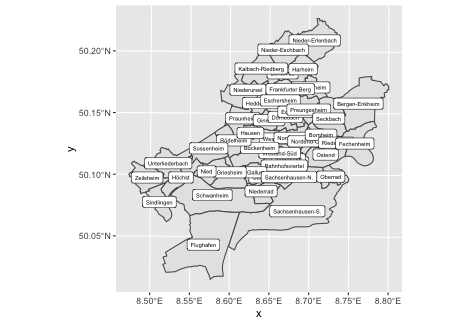
\includegraphics{_main_files/figure-latex/unnamed-chunk-71-1.png}

\hypertarget{osm-daten}{%
\subsection{OSM-Daten}\label{osm-daten}}

Im \href{https://wiki.openstreetmap.org/wiki/Map_Features}{OSM Wiki} suchen wir den richtigen \emph{tag} heraus. In diesem Fall \texttt{shop=kiosk}

Dann bauen wir auf \href{https://overpass-turbo.eu/}{Overpass Turbo} die Abfrage und laden den Datensatz herunter.

Schließlich importieren wir:

\begin{Shaded}
\begin{Highlighting}[]
\NormalTok{kioske }\OtherTok{\textless{}{-}} \FunctionTok{st\_read}\NormalTok{(}\StringTok{"resources/kioske.geojson"}\NormalTok{)}
\DocumentationTok{\#\# Reading layer \textasciigrave{}kioske\textquotesingle{} from data source }
\DocumentationTok{\#\#   \textasciigrave{}/Users/till/mzs/2021\_methodenwoche/skript/resources/kioske.geojson\textquotesingle{} }
\DocumentationTok{\#\#   using driver \textasciigrave{}GeoJSON\textquotesingle{}}
\DocumentationTok{\#\# Simple feature collection with 325 features and 74 fields}
\DocumentationTok{\#\# Geometry type: GEOMETRY}
\DocumentationTok{\#\# Dimension:     XY}
\DocumentationTok{\#\# Bounding box:  xmin: 8.505468 ymin: 50.04801 xmax: 8.789538 ymax: 50.20185}
\DocumentationTok{\#\# Geodetic CRS:  WGS 84}
\end{Highlighting}
\end{Shaded}

Eine Vorschau:

\begin{Shaded}
\begin{Highlighting}[]
\FunctionTok{ggplot}\NormalTok{() }\SpecialCharTok{+}
  \FunctionTok{geom\_sf}\NormalTok{(}\AttributeTok{data =}\NormalTok{ stadtteile) }\SpecialCharTok{+}
  \FunctionTok{geom\_sf}\NormalTok{(}\AttributeTok{data =}\NormalTok{ kioske)}
\end{Highlighting}
\end{Shaded}

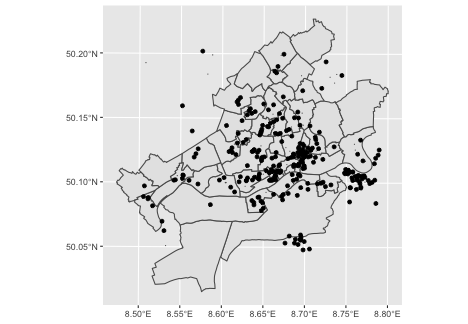
\includegraphics{_main_files/figure-latex/unnamed-chunk-73-1.png}

\hypertarget{koordinatenreferenzsysteme}{%
\subsection{Koordinatenreferenzsysteme}\label{koordinatenreferenzsysteme}}

Der OSM-Datensatz ist mit WGS84 (EPSG 4326) referenziert:

\begin{Shaded}
\begin{Highlighting}[]
\FunctionTok{st\_crs}\NormalTok{(kioske)}
\DocumentationTok{\#\# Coordinate Reference System:}
\DocumentationTok{\#\#   User input: WGS 84 }
\DocumentationTok{\#\#   wkt:}
\DocumentationTok{\#\# GEOGCRS["WGS 84",}
\DocumentationTok{\#\#     DATUM["World Geodetic System 1984",}
\DocumentationTok{\#\#         ELLIPSOID["WGS 84",6378137,298.257223563,}
\DocumentationTok{\#\#             LENGTHUNIT["metre",1]]],}
\DocumentationTok{\#\#     PRIMEM["Greenwich",0,}
\DocumentationTok{\#\#         ANGLEUNIT["degree",0.0174532925199433]],}
\DocumentationTok{\#\#     CS[ellipsoidal,2],}
\DocumentationTok{\#\#         AXIS["geodetic latitude (Lat)",north,}
\DocumentationTok{\#\#             ORDER[1],}
\DocumentationTok{\#\#             ANGLEUNIT["degree",0.0174532925199433]],}
\DocumentationTok{\#\#         AXIS["geodetic longitude (Lon)",east,}
\DocumentationTok{\#\#             ORDER[2],}
\DocumentationTok{\#\#             ANGLEUNIT["degree",0.0174532925199433]],}
\DocumentationTok{\#\#     ID["EPSG",4326]]}
\end{Highlighting}
\end{Shaded}

Die Stadtteilen hingegen sind sind in ETSR89 (EPSG 25832):

\begin{Shaded}
\begin{Highlighting}[]
\FunctionTok{st\_crs}\NormalTok{(stadtteile)}
\DocumentationTok{\#\# Coordinate Reference System:}
\DocumentationTok{\#\#   User input: ETRS89 / UTM zone 32N }
\DocumentationTok{\#\#   wkt:}
\DocumentationTok{\#\# PROJCRS["ETRS89 / UTM zone 32N",}
\DocumentationTok{\#\#     BASEGEOGCRS["ETRS89",}
\DocumentationTok{\#\#         DATUM["European Terrestrial Reference System 1989",}
\DocumentationTok{\#\#             ELLIPSOID["GRS 1980",6378137,298.257222101,}
\DocumentationTok{\#\#                 LENGTHUNIT["metre",1]]],}
\DocumentationTok{\#\#         PRIMEM["Greenwich",0,}
\DocumentationTok{\#\#             ANGLEUNIT["degree",0.0174532925199433]],}
\DocumentationTok{\#\#         ID["EPSG",4258]],}
\DocumentationTok{\#\#     CONVERSION["UTM zone 32N",}
\DocumentationTok{\#\#         METHOD["Transverse Mercator",}
\DocumentationTok{\#\#             ID["EPSG",9807]],}
\DocumentationTok{\#\#         PARAMETER["Latitude of natural origin",0,}
\DocumentationTok{\#\#             ANGLEUNIT["degree",0.0174532925199433],}
\DocumentationTok{\#\#             ID["EPSG",8801]],}
\DocumentationTok{\#\#         PARAMETER["Longitude of natural origin",9,}
\DocumentationTok{\#\#             ANGLEUNIT["degree",0.0174532925199433],}
\DocumentationTok{\#\#             ID["EPSG",8802]],}
\DocumentationTok{\#\#         PARAMETER["Scale factor at natural origin",0.9996,}
\DocumentationTok{\#\#             SCALEUNIT["unity",1],}
\DocumentationTok{\#\#             ID["EPSG",8805]],}
\DocumentationTok{\#\#         PARAMETER["False easting",500000,}
\DocumentationTok{\#\#             LENGTHUNIT["metre",1],}
\DocumentationTok{\#\#             ID["EPSG",8806]],}
\DocumentationTok{\#\#         PARAMETER["False northing",0,}
\DocumentationTok{\#\#             LENGTHUNIT["metre",1],}
\DocumentationTok{\#\#             ID["EPSG",8807]]],}
\DocumentationTok{\#\#     CS[Cartesian,2],}
\DocumentationTok{\#\#         AXIS["(E)",east,}
\DocumentationTok{\#\#             ORDER[1],}
\DocumentationTok{\#\#             LENGTHUNIT["metre",1]],}
\DocumentationTok{\#\#         AXIS["(N)",north,}
\DocumentationTok{\#\#             ORDER[2],}
\DocumentationTok{\#\#             LENGTHUNIT["metre",1]],}
\DocumentationTok{\#\#     USAGE[}
\DocumentationTok{\#\#         SCOPE["Engineering survey, topographic mapping."],}
\DocumentationTok{\#\#         AREA["Europe between 6°E and 12°E: Austria; Belgium; Denmark {-} onshore and offshore; Germany {-} onshore and offshore; Norway including {-} onshore and offshore; Spain {-} offshore."],}
\DocumentationTok{\#\#         BBOX[38.76,6,83.92,12]],}
\DocumentationTok{\#\#     ID["EPSG",25832]]}
\end{Highlighting}
\end{Shaded}

Der Datensatz lässt sich allerdings transformieren:

\begin{Shaded}
\begin{Highlighting}[]
\NormalTok{stadtteile }\SpecialCharTok{\%\textgreater{}\%}
  \FunctionTok{st\_transform}\NormalTok{(}\DecValTok{4326}\NormalTok{) }\SpecialCharTok{\%\textgreater{}\%}
  \FunctionTok{st\_crs}\NormalTok{()}
\DocumentationTok{\#\# Coordinate Reference System:}
\DocumentationTok{\#\#   User input: EPSG:4326 }
\DocumentationTok{\#\#   wkt:}
\DocumentationTok{\#\# GEOGCRS["WGS 84",}
\DocumentationTok{\#\#     DATUM["World Geodetic System 1984",}
\DocumentationTok{\#\#         ELLIPSOID["WGS 84",6378137,298.257223563,}
\DocumentationTok{\#\#             LENGTHUNIT["metre",1]]],}
\DocumentationTok{\#\#     PRIMEM["Greenwich",0,}
\DocumentationTok{\#\#         ANGLEUNIT["degree",0.0174532925199433]],}
\DocumentationTok{\#\#     CS[ellipsoidal,2],}
\DocumentationTok{\#\#         AXIS["geodetic latitude (Lat)",north,}
\DocumentationTok{\#\#             ORDER[1],}
\DocumentationTok{\#\#             ANGLEUNIT["degree",0.0174532925199433]],}
\DocumentationTok{\#\#         AXIS["geodetic longitude (Lon)",east,}
\DocumentationTok{\#\#             ORDER[2],}
\DocumentationTok{\#\#             ANGLEUNIT["degree",0.0174532925199433]],}
\DocumentationTok{\#\#     USAGE[}
\DocumentationTok{\#\#         SCOPE["Horizontal component of 3D system."],}
\DocumentationTok{\#\#         AREA["World."],}
\DocumentationTok{\#\#         BBOX[{-}90,{-}180,90,180]],}
\DocumentationTok{\#\#     ID["EPSG",4326]]}
\end{Highlighting}
\end{Shaded}

Jetzt haben beide Datensätze den selben EPSG-Code. Das ist die Voraussetzung für den nächsten Schritt.

\hypertarget{verschneiden}{%
\subsection{Verschneiden}\label{verschneiden}}

Mit \texttt{st\_covers()} und \texttt{lengths()} lassen sich die Anzahl der Kioske in jedem Stadtteil zählen und einer neuen Spalte im Originaldatensatz zuordnen:

\begin{Shaded}
\begin{Highlighting}[]
\NormalTok{stadtteile }\SpecialCharTok{\%\textgreater{}\%}
  \FunctionTok{st\_transform}\NormalTok{(}\DecValTok{4326}\NormalTok{) }\SpecialCharTok{\%\textgreater{}\%}
  \FunctionTok{st\_covers}\NormalTok{(kioske) }\SpecialCharTok{\%\textgreater{}\%}
  \FunctionTok{lengths}\NormalTok{() }\OtherTok{{-}\textgreater{}}\NormalTok{ stadtteile}\SpecialCharTok{$}\NormalTok{anzahl\_kioske}
\end{Highlighting}
\end{Shaded}

Auf einer Karte veranschaulicht:

\begin{Shaded}
\begin{Highlighting}[]
\FunctionTok{ggplot}\NormalTok{(stadtteile) }\SpecialCharTok{+}
  \FunctionTok{geom\_sf}\NormalTok{(}\FunctionTok{aes}\NormalTok{(}\AttributeTok{fill =}\NormalTok{ anzahl\_kioske))}
\end{Highlighting}
\end{Shaded}

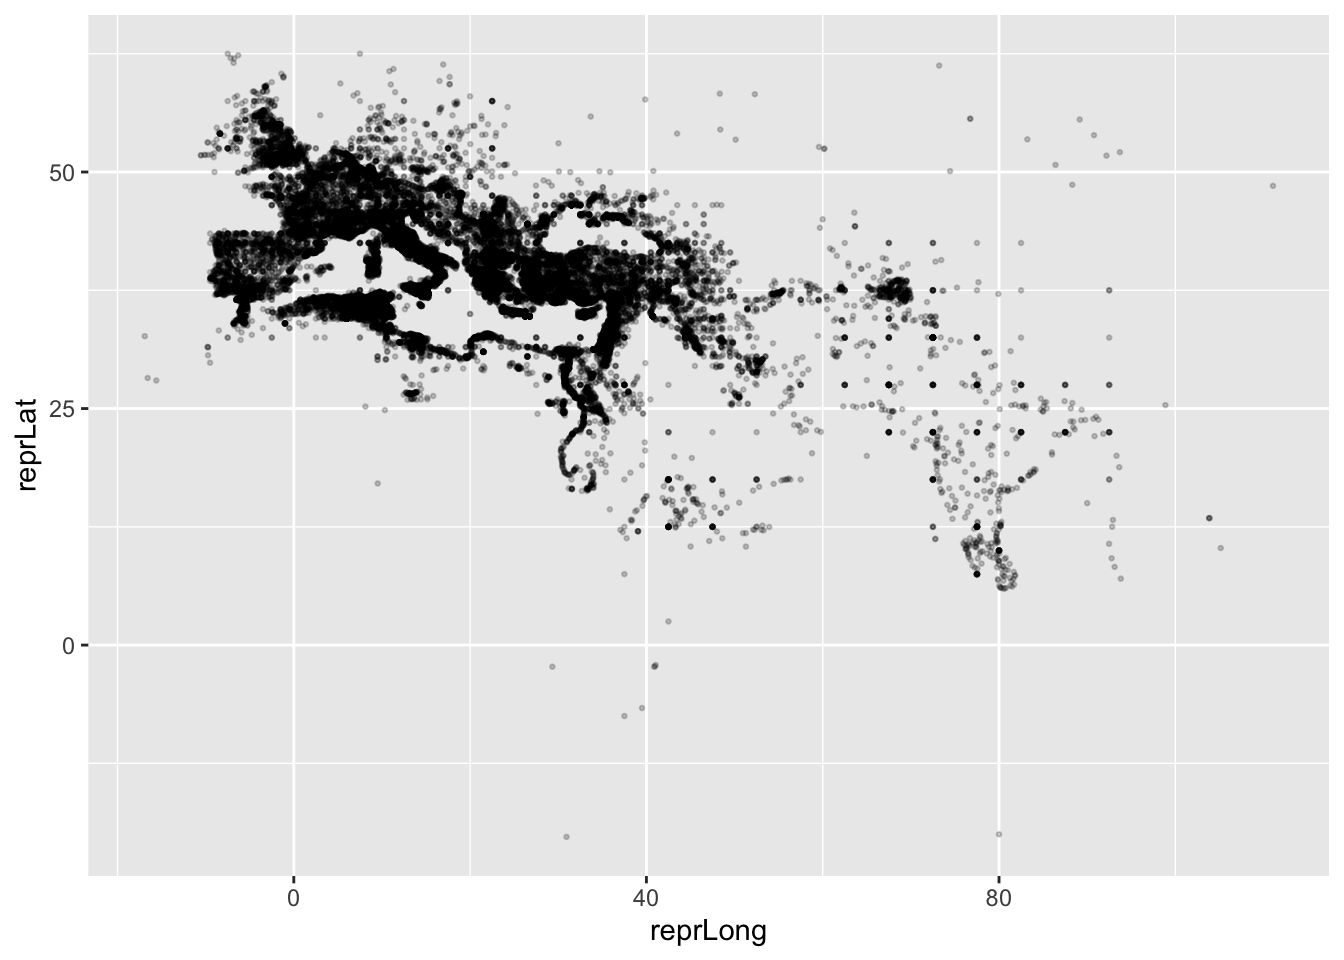
\includegraphics{_main_files/figure-latex/unnamed-chunk-78-1.png}

Allerdings wäre es schöner, die Kioskdichte (nach Fläche) darzustellen. Dazu berechnen wir zunächst die Flächen der Stadtteile:

\begin{Shaded}
\begin{Highlighting}[]
\FunctionTok{st\_area}\NormalTok{(stadtteile) }\SpecialCharTok{\%\textgreater{}\%}
  \FunctionTok{as.numeric}\NormalTok{() }\SpecialCharTok{/} \DecValTok{1000} \SpecialCharTok{/} \DecValTok{1000} \OtherTok{{-}\textgreater{}}
\NormalTok{  stadtteile}\SpecialCharTok{$}\NormalTok{qkm}
\end{Highlighting}
\end{Shaded}

Oder mit Pipes:

\begin{Shaded}
\begin{Highlighting}[]
\NormalTok{stadtteile }\SpecialCharTok{\%\textgreater{}\%}
  \FunctionTok{mutate}\NormalTok{(}\AttributeTok{qkm =} \FunctionTok{st\_area}\NormalTok{(.) }\SpecialCharTok{\%\textgreater{}\%} \FunctionTok{as.numeric}\NormalTok{() }\SpecialCharTok{/} \DecValTok{1000} \SpecialCharTok{/} \DecValTok{1000}\NormalTok{)}
\DocumentationTok{\#\# Simple feature collection with 46 features and 4 fields}
\DocumentationTok{\#\# Geometry type: POLYGON}
\DocumentationTok{\#\# Dimension:     XY}
\DocumentationTok{\#\# Bounding box:  xmin: 462292.7 ymin: 5540412 xmax: 485744.8 ymax: 5563925}
\DocumentationTok{\#\# Projected CRS: ETRS89 / UTM zone 32N}
\DocumentationTok{\#\# First 10 features:}
\DocumentationTok{\#\#    STTLNR        STTLNAME                       geometry anzahl\_kioske}
\DocumentationTok{\#\# 1       1        Altstadt POLYGON ((476934.3 5550541,...             5}
\DocumentationTok{\#\# 2       2      Innenstadt POLYGON ((477611.9 5552034,...             5}
\DocumentationTok{\#\# 3       3 Bahnhofsviertel POLYGON ((475831 5550785, 4...             7}
\DocumentationTok{\#\# 4       4     Westend{-}Süd POLYGON ((475745.4 5552373,...             6}
\DocumentationTok{\#\# 5       5    Westend{-}Nord POLYGON ((476497.9 5553910,...             3}
\DocumentationTok{\#\# 6       6    Nordend{-}West POLYGON ((478362.5 5553898,...            10}
\DocumentationTok{\#\# 7       7     Nordend{-}Ost POLYGON ((478397.9 5551924,...            17}
\DocumentationTok{\#\# 8       8          Ostend POLYGON ((481955.2 5552141,...            15}
\DocumentationTok{\#\# 9       9        Bornheim POLYGON ((478959.8 5552336,...            14}
\DocumentationTok{\#\# 10     10  Gutleutviertel POLYGON ((472942 5548802, 4...            11}
\DocumentationTok{\#\#          qkm}
\DocumentationTok{\#\# 1  0.5065673}
\DocumentationTok{\#\# 2  1.4902009}
\DocumentationTok{\#\# 3  0.5425421}
\DocumentationTok{\#\# 4  2.4948957}
\DocumentationTok{\#\# 5  1.6307925}
\DocumentationTok{\#\# 6  3.0977694}
\DocumentationTok{\#\# 7  1.5305338}
\DocumentationTok{\#\# 8  5.5573382}
\DocumentationTok{\#\# 9  2.7840413}
\DocumentationTok{\#\# 10 2.1982354}
\end{Highlighting}
\end{Shaded}

Und dann die Kioskdichte:

\begin{Shaded}
\begin{Highlighting}[]
\NormalTok{stadtteile }\SpecialCharTok{\%\textgreater{}\%}
  \FunctionTok{mutate}\NormalTok{(}\AttributeTok{qkm =} \FunctionTok{st\_area}\NormalTok{(.) }\SpecialCharTok{\%\textgreater{}\%} \FunctionTok{as.numeric}\NormalTok{() }\SpecialCharTok{/} \DecValTok{1000} \SpecialCharTok{/} \DecValTok{1000}\NormalTok{,}
         \AttributeTok{kioskdichte =}\NormalTok{ anzahl\_kioske }\SpecialCharTok{/}\NormalTok{ qkm)}
\DocumentationTok{\#\# Simple feature collection with 46 features and 5 fields}
\DocumentationTok{\#\# Geometry type: POLYGON}
\DocumentationTok{\#\# Dimension:     XY}
\DocumentationTok{\#\# Bounding box:  xmin: 462292.7 ymin: 5540412 xmax: 485744.8 ymax: 5563925}
\DocumentationTok{\#\# Projected CRS: ETRS89 / UTM zone 32N}
\DocumentationTok{\#\# First 10 features:}
\DocumentationTok{\#\#    STTLNR        STTLNAME                       geometry anzahl\_kioske}
\DocumentationTok{\#\# 1       1        Altstadt POLYGON ((476934.3 5550541,...             5}
\DocumentationTok{\#\# 2       2      Innenstadt POLYGON ((477611.9 5552034,...             5}
\DocumentationTok{\#\# 3       3 Bahnhofsviertel POLYGON ((475831 5550785, 4...             7}
\DocumentationTok{\#\# 4       4     Westend{-}Süd POLYGON ((475745.4 5552373,...             6}
\DocumentationTok{\#\# 5       5    Westend{-}Nord POLYGON ((476497.9 5553910,...             3}
\DocumentationTok{\#\# 6       6    Nordend{-}West POLYGON ((478362.5 5553898,...            10}
\DocumentationTok{\#\# 7       7     Nordend{-}Ost POLYGON ((478397.9 5551924,...            17}
\DocumentationTok{\#\# 8       8          Ostend POLYGON ((481955.2 5552141,...            15}
\DocumentationTok{\#\# 9       9        Bornheim POLYGON ((478959.8 5552336,...            14}
\DocumentationTok{\#\# 10     10  Gutleutviertel POLYGON ((472942 5548802, 4...            11}
\DocumentationTok{\#\#          qkm kioskdichte}
\DocumentationTok{\#\# 1  0.5065673    9.870357}
\DocumentationTok{\#\# 2  1.4902009    3.355252}
\DocumentationTok{\#\# 3  0.5425421   12.902225}
\DocumentationTok{\#\# 4  2.4948957    2.404910}
\DocumentationTok{\#\# 5  1.6307925    1.839596}
\DocumentationTok{\#\# 6  3.0977694    3.228129}
\DocumentationTok{\#\# 7  1.5305338   11.107236}
\DocumentationTok{\#\# 8  5.5573382    2.699134}
\DocumentationTok{\#\# 9  2.7840413    5.028661}
\DocumentationTok{\#\# 10 2.1982354    5.004014}
\end{Highlighting}
\end{Shaded}

Schließlich die Karte:

\begin{Shaded}
\begin{Highlighting}[]
\NormalTok{stadtteile }\SpecialCharTok{\%\textgreater{}\%}
  \FunctionTok{mutate}\NormalTok{(}\AttributeTok{qkm =} \FunctionTok{st\_area}\NormalTok{(.) }\SpecialCharTok{\%\textgreater{}\%} \FunctionTok{as.numeric}\NormalTok{() }\SpecialCharTok{/} \DecValTok{1000} \SpecialCharTok{/} \DecValTok{1000}\NormalTok{,}
         \AttributeTok{kioskdichte =}\NormalTok{ anzahl\_kioske }\SpecialCharTok{/}\NormalTok{ qkm) }\SpecialCharTok{\%\textgreater{}\%}
  \FunctionTok{ggplot}\NormalTok{() }\SpecialCharTok{+}
    \FunctionTok{geom\_sf}\NormalTok{(}\FunctionTok{aes}\NormalTok{(}\AttributeTok{fill =}\NormalTok{ kioskdichte), }\AttributeTok{color=}\ConstantTok{NA}\NormalTok{) }\SpecialCharTok{+}
    \FunctionTok{scale\_fill\_continuous}\NormalTok{(}\StringTok{"Kioske pro km²"}\NormalTok{) }\SpecialCharTok{+}
    \FunctionTok{theme\_void}\NormalTok{()}
\end{Highlighting}
\end{Shaded}

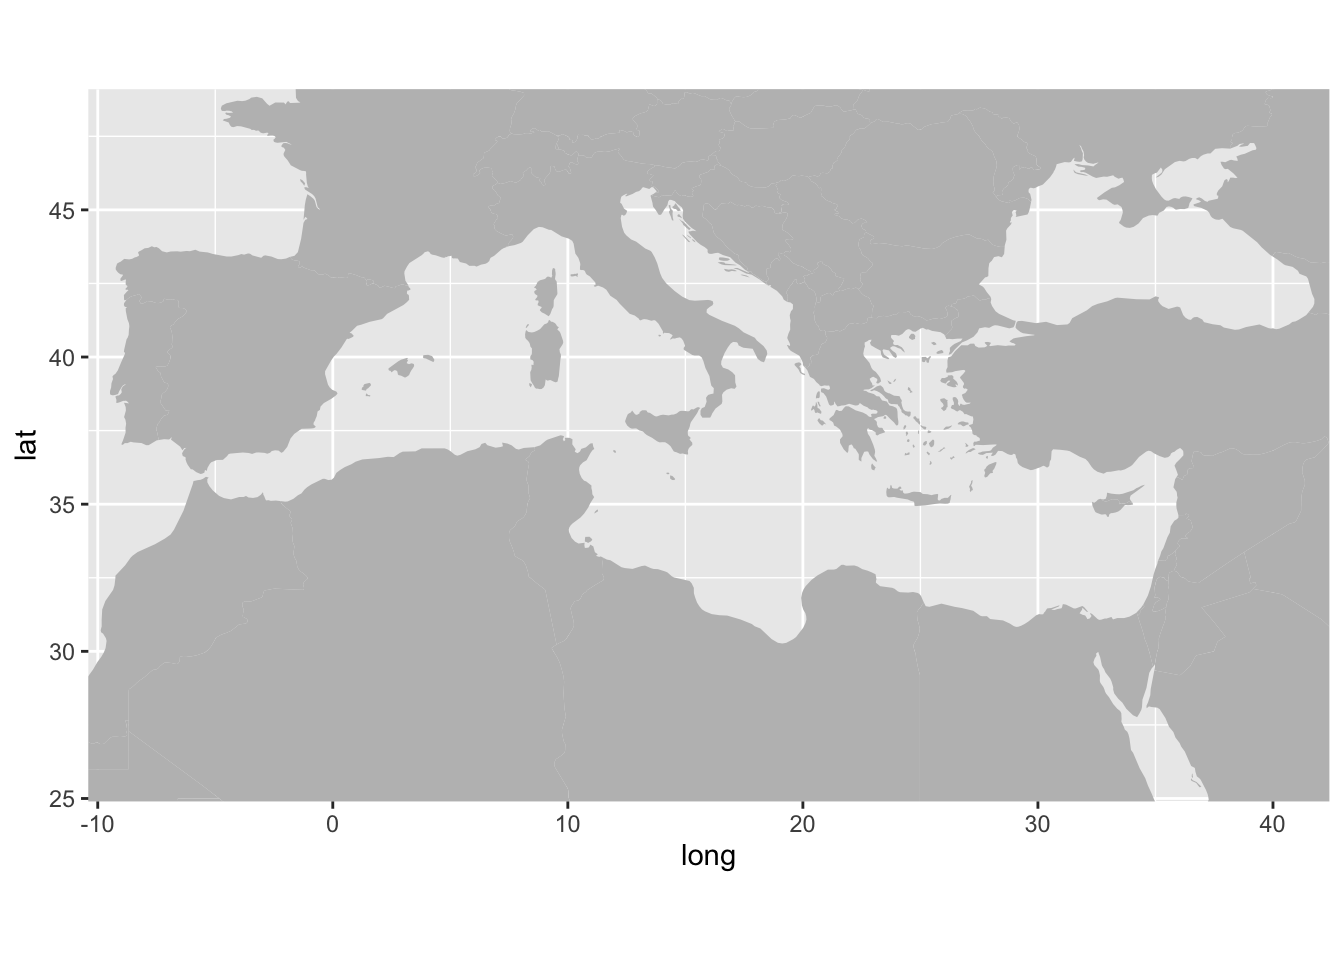
\includegraphics{_main_files/figure-latex/unnamed-chunk-82-1.png}

\hypertarget{aufgaben-3}{%
\subsection{Aufgaben}\label{aufgaben-3}}

\begin{enumerate}
\def\labelenumi{\arabic{enumi}.}
\item
  Erstellen Sie eine Choroplethenkarte der Frankfurter Stadtteile, in der Sie die Anzahl bzw. die Dichte von Apotheken darstellen. (Schritte analog zu oben.)
\item
  Welche Stadtteile haben mehr Kioske? Welche mehr Apotheken? Wie ausgeprägt ist das Verhältnis? Erstellen Sie eine Karte, die das zum Ausdruck bringt.
\item
  (Achtung, knifflig!) Siemens veröffentlicht einen \href{https://press.siemens.com/global/de/feature/wo-blitzt-es-am-haeufigsten}{Blitzatlas}. Laden Sie den Datensatz herunter und bauen Sie die folgende Ansicht nach:

  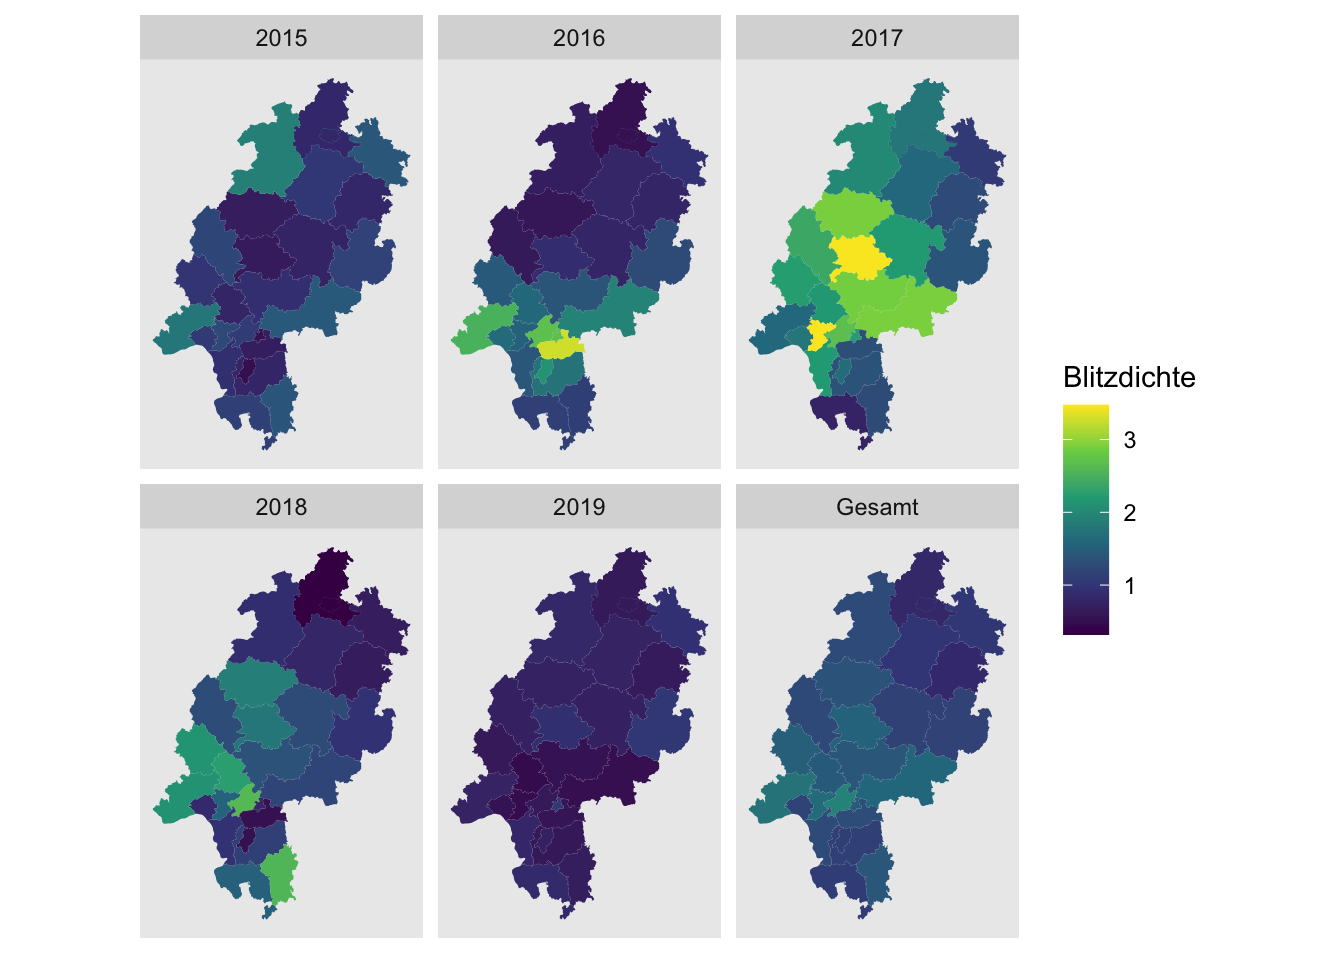
\includegraphics{_main_files/figure-latex/unnamed-chunk-86-1.png}
\end{enumerate}

\hypertarget{weitere-methoden}{%
\section{Weitere Methoden}\label{weitere-methoden}}

\hypertarget{vorbereitung-2}{%
\subsection{Vorbereitung}\label{vorbereitung-2}}

Für diese Lektion brauchen wir folgende Pakete:

\begin{Shaded}
\begin{Highlighting}[]
\FunctionTok{library}\NormalTok{(tidyverse)}
\FunctionTok{library}\NormalTok{(sf)}
\FunctionTok{library}\NormalTok{(tmap)}
\end{Highlighting}
\end{Shaded}

\hypertarget{aufgabe}{%
\subsection{Aufgabe}\label{aufgabe}}

Ziel soll sein, eine Deutschlandkarte mit Tankstellenpreisen für Diesel zu erstellen.

\hypertarget{daten-einlesen}{%
\subsection{Daten einlesen}\label{daten-einlesen}}

Das ``Tankerkönig''-Projekt veröffentlicht aktuelle Tankstellenpreise über eine API, und stellt historische Preise hier bereit: \url{https://dev.azure.com/tankerkoenig/_git/tankerkoenig-data}

Wir laden die Dateien für \texttt{prices} und \texttt{stations} von einem Tag (hier: 26.5.2019) herunter und speichern sie im Unterordner \texttt{resources} des Projektordners.

Dann können wir sie einlesen:

\begin{Shaded}
\begin{Highlighting}[]
\NormalTok{preise }\OtherTok{\textless{}{-}} \FunctionTok{read\_csv}\NormalTok{(}\StringTok{"resources/2019{-}05{-}26{-}prices.csv"}\NormalTok{)}
\NormalTok{preise}
\end{Highlighting}
\end{Shaded}

\begin{verbatim}
## # A tibble: 231,174 x 8
##    date                station_uuid     diesel    e5   e10 dieselchange e5change
##    <dttm>              <chr>             <dbl> <dbl> <dbl>        <dbl>    <dbl>
##  1 2019-05-25 22:01:06 51e171d0-1a9c-4~   1.37  1.58  1.56            1        1
##  2 2019-05-25 22:02:06 8a796af1-8d78-4~   1.32  1.56  1.54            1        1
##  3 2019-05-25 22:02:06 2d658127-11b5-4~   1.28  1.52  0               0        1
##  4 2019-05-25 22:03:06 904d3a45-df30-4~   1.32  1.54  1.52            1        1
##  5 2019-05-25 22:03:06 a98ed5d0-261b-4~   1.34  1.57  1.55            1        1
##  6 2019-05-25 22:04:06 7671d5ad-4c7d-4~   1.30  1.54  0               1        1
##  7 2019-05-25 22:04:06 44fa4d12-5571-4~   1.34  1.58  1.56            1        1
##  8 2019-05-25 22:04:06 da9abcda-3218-4~   1.38  1.52  1.50            0        1
##  9 2019-05-25 22:04:06 bcba0c2b-fbe7-4~   1.35  1.55  1.53            0        1
## 10 2019-05-25 22:04:06 00061000-0001-4~   1.20  1.48  1.46            1        1
## # ... with 231,164 more rows, and 1 more variable: e10change <dbl>
\end{verbatim}

\hypertarget{uxfcberblick-verschaffen-1}{%
\subsection{Überblick verschaffen}\label{uxfcberblick-verschaffen-1}}

Beim nähreren Betrachten fällt auf, dass im Datensatz \texttt{preise} 231.174 Zeilen enthalten sind, in \texttt{stations} nur 15.668. Das liegt daran, das für jede Station \emph{mehrere} Preisupdates im Datensatz \texttt{preise} stehen, jedoch nur \emph{einmal} die gleichbleibenden Informationen (Name, Marke, Adresse, Koordinaten) in \texttt{stations}.

Beide Datensätze sind über einen eindeutigen „Key`` verbunden: In \texttt{preise} heißt er \texttt{station\_uuid}, in \texttt{stations} einfach nur \texttt{uuid}.

Um ein besseres Gefühl für den Datensatz zu bekommen, könnten wir uns z.~B. anschauen, zu welcher Uhrzeit wie viele Preise aktualisiert wurden:

\begin{Shaded}
\begin{Highlighting}[]
\FunctionTok{ggplot}\NormalTok{(preise) }\SpecialCharTok{+}
  \FunctionTok{geom\_histogram}\NormalTok{(}\FunctionTok{aes}\NormalTok{(}\AttributeTok{x =}\NormalTok{ date))}
\end{Highlighting}
\end{Shaded}

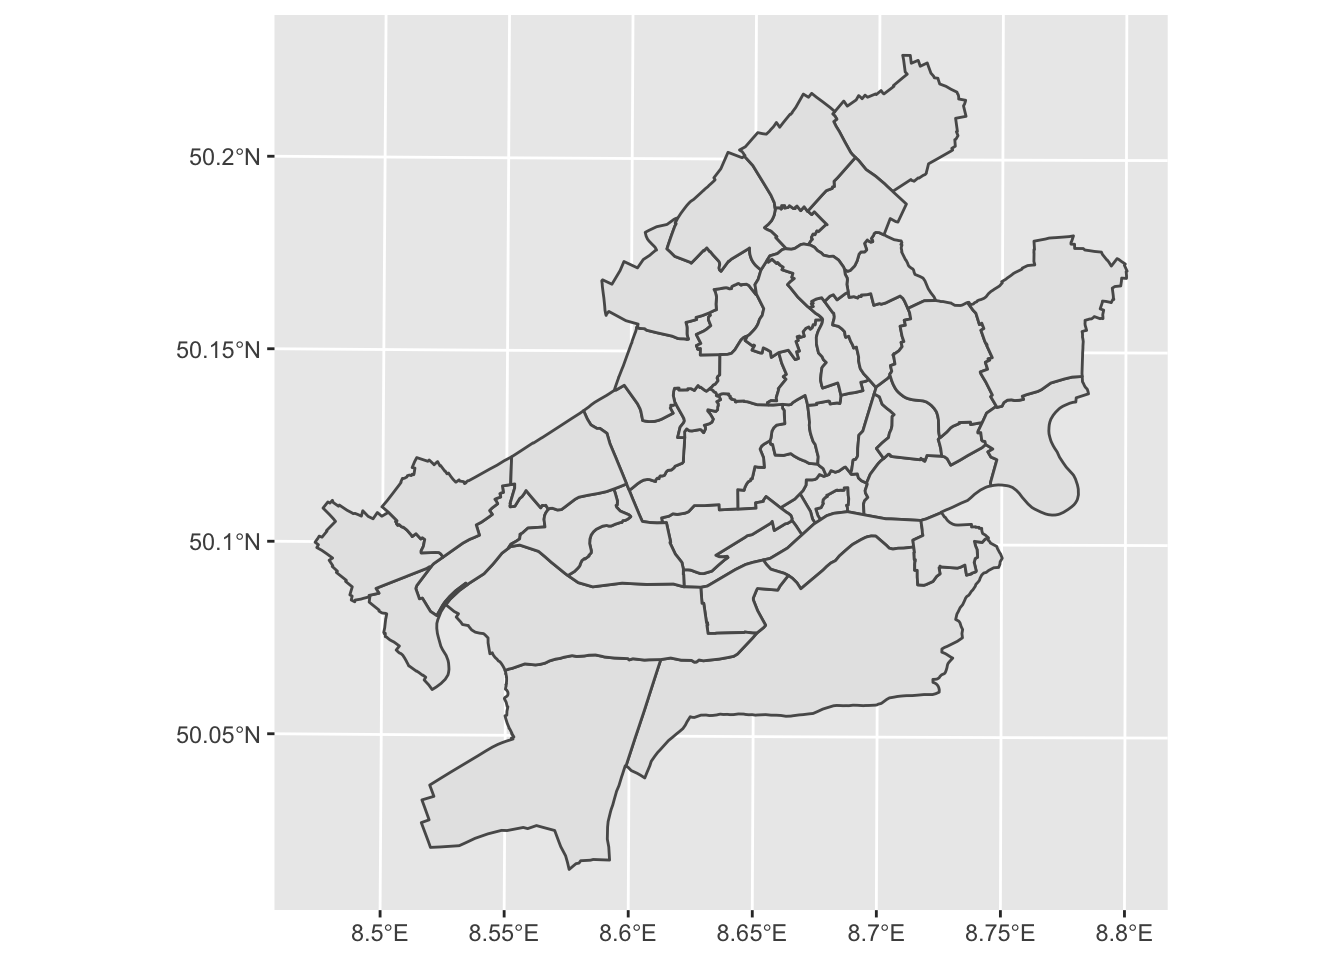
\includegraphics{_main_files/figure-latex/unnamed-chunk-90-1.png}

\hypertarget{zusammenfassen}{%
\subsection{Zusammenfassen}\label{zusammenfassen}}

Eine weitere Frage könnte sein: Wie sieht die Verteilung der Anzahl der Preisupdates je Tankstelle aus? Hierfür müssen wir den Datensatz \texttt{preise} anhand der Spalte \texttt{station\_uuid} zusammenfassen und die Einträge zählen. Das geht mit \texttt{group\_by()} und \texttt{summarize()}:

\begin{Shaded}
\begin{Highlighting}[]
\NormalTok{preise }\SpecialCharTok{\%\textgreater{}\%}
  \FunctionTok{group\_by}\NormalTok{(station\_uuid) }\SpecialCharTok{\%\textgreater{}\%}
  \FunctionTok{summarize}\NormalTok{(}\AttributeTok{anzahl\_updates =} \FunctionTok{n}\NormalTok{()) }\SpecialCharTok{\%\textgreater{}\%}
  \FunctionTok{ggplot}\NormalTok{() }\SpecialCharTok{+}
    \FunctionTok{geom\_histogram}\NormalTok{(}\FunctionTok{aes}\NormalTok{(}\AttributeTok{x =}\NormalTok{ anzahl\_updates))}
\end{Highlighting}
\end{Shaded}

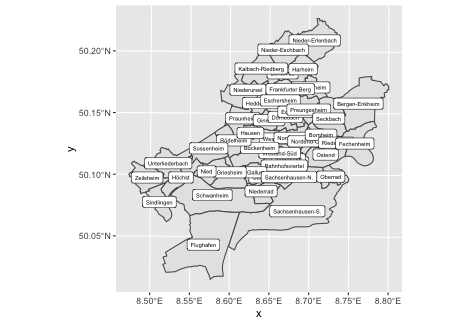
\includegraphics{_main_files/figure-latex/unnamed-chunk-91-1.png}

Um unserem Ziel der Dieselkarte etwas näher zu kommen, sollten wir aber nicht die Anzahl der Updates zusammenfassen, sondern den Dieselpreis.
Aber nach welchem Schema?
Einfach nur den Durchschnitt (mit \texttt{mean()}) zu nehmen, könnte das Bild verfälschen: Man stelle sich z.~B. vor, ein besonders teurer (oder günstiger) Preis sei nur wenige Sekunden gültig gewesen.

Wir orientieren uns einfach an der Börse und nehmen einfach den letzten gültigen Preis (wie der Aktienwert bei Börsenschluss).
Dafür müssen wir den Datensatz erst mit \texttt{arrange()} chronologisch sortieren, dann entsprechend gruppieren und mit \texttt{last()} zusammenfassen:

\begin{Shaded}
\begin{Highlighting}[]
\NormalTok{preise }\SpecialCharTok{\%\textgreater{}\%}
  \FunctionTok{arrange}\NormalTok{(date) }\SpecialCharTok{\%\textgreater{}\%}
  \FunctionTok{group\_by}\NormalTok{(station\_uuid) }\SpecialCharTok{\%\textgreater{}\%}
  \FunctionTok{summarize}\NormalTok{(}\AttributeTok{dieselpreis =} \FunctionTok{last}\NormalTok{(diesel),}
            \AttributeTok{e5preis     =} \FunctionTok{last}\NormalTok{(e5),}
            \AttributeTok{e10preis    =} \FunctionTok{last}\NormalTok{(e10)) }\OtherTok{{-}\textgreater{}}
\NormalTok{  preise\_nach\_tankstelle}

\NormalTok{preise\_nach\_tankstelle}
\DocumentationTok{\#\# \# A tibble: 13,701 x 4}
\DocumentationTok{\#\#    station\_uuid                         dieselpreis e5preis e10preis}
\DocumentationTok{\#\#    \textless{}chr\textgreater{}                                      \textless{}dbl\textgreater{}   \textless{}dbl\textgreater{}    \textless{}dbl\textgreater{}}
\DocumentationTok{\#\#  1 00006210{-}0037{-}4444{-}8888{-}acdc00006210        1.33    1.55     1.53}
\DocumentationTok{\#\#  2 00016899{-}3247{-}4444{-}8888{-}acdc00000007        1.31    1.53     1.51}
\DocumentationTok{\#\#  3 00060001{-}d387{-}4444{-}8888{-}acdc00000001        1.37    1.62     1.60}
\DocumentationTok{\#\#  4 00060009{-}3adf{-}4444{-}8888{-}acdc00000001        1.35    1.64     1.62}
\DocumentationTok{\#\#  5 00060014{-}b0d9{-}4444{-}8888{-}acdc00000002        1.32    1.61     1.59}
\DocumentationTok{\#\#  6 00060015{-}0090{-}4444{-}8888{-}acdc00000090        1.27    1.52     1.50}
\DocumentationTok{\#\#  7 00060016{-}ed96{-}4444{-}8888{-}acdc00000001        1.35    1.57     1.55}
\DocumentationTok{\#\#  8 00060034{-}0011{-}4444{-}8888{-}acdc00000011        1.37    1.61     1.59}
\DocumentationTok{\#\#  9 00060051{-}533e{-}75a1{-}87f9{-}8a9f00060051        1.25    1.50     1.48}
\DocumentationTok{\#\# 10 00060055{-}0001{-}4444{-}8888{-}acdc00000001        1.26    1.53     1.51}
\DocumentationTok{\#\# \# ... with 13,691 more rows}
\end{Highlighting}
\end{Shaded}

\hypertarget{verschneiden-1}{%
\subsection{Verschneiden}\label{verschneiden-1}}

Jetzt haben wir für jede Station nur noch eine Zeile mit den Preisen.
Um das zu kartieren, fehlen noch die Informationen zu den Tankstellen. Dafür laden wir auch den \texttt{stations}-Datensatz für den richtigen Tag herunter und importieren ihn in R:

\begin{Shaded}
\begin{Highlighting}[]
\NormalTok{tankstellen }\OtherTok{\textless{}{-}} \FunctionTok{read\_csv}\NormalTok{(}\StringTok{"resources/2019{-}05{-}26{-}stations.csv"}\NormalTok{)}
\NormalTok{tankstellen}
\end{Highlighting}
\end{Shaded}

\begin{verbatim}
## # A tibble: 15,668 x 11
##    uuid    name    brand  street house_number post_code city  latitude longitude
##    <chr>   <chr>   <chr>  <chr>  <chr>        <chr>     <chr>    <dbl>     <dbl>
##  1 0e18d0~ OIL! T~ OIL!   Evers~ <NA>         80999     Münc~     48.2     11.5 
##  2 ad8122~ bft Bo~ bft    Godes~ 55           53175     Bonn      50.7      7.14
##  3 44e2bd~ bft Ta~ <NA>   Schel~ 53           36304     Alsf~     50.8      9.28
##  4 1a8e4d~ Hessol  Hessol Frank~ 65           61279     Gräv~     50.4      8.46
##  5 005056~ star T~ STAR   Leipz~ 11           06217     Mers~     51.4     12.0 
##  6 d435f7~ ROSDOR~ Shell  A7 GÖ~ <NA>         37124     Rosd~     51.5      9.88
##  7 88a23d~ AVIA T~ AVIA   Burgs~ 8            63637     Joss~     50.2      9.48
##  8 f0e93f~ Aral T~ ARAL   Eicke~ 357          41063     Mönc~     51.2      6.45
##  9 005056~ star T~ STAR   Celle~ 55           29303     Berg~     52.8      9.97
## 10 8e47dd~ Aral T~ ARAL   Crail~ 32           74532     Ilsh~     49.2      9.93
## # ... with 15,658 more rows, and 2 more variables: first_active <dttm>,
## #   openingtimes_json <chr>
\end{verbatim}

Wir verschneiden mit \texttt{inner\_join()} unter Angabe der relevanten Spaltennamen und wählen die Spalten aus, mit denen wir weiterarbeiten wollen:

\begin{Shaded}
\begin{Highlighting}[]
\FunctionTok{inner\_join}\NormalTok{(preise\_nach\_tankstelle, tankstellen,}
           \AttributeTok{by =} \FunctionTok{c}\NormalTok{(}\StringTok{"station\_uuid"} \OtherTok{=} \StringTok{"uuid"}\NormalTok{)) }\SpecialCharTok{\%\textgreater{}\%}
  \FunctionTok{select}\NormalTok{(dieselpreis, e5preis, e10preis, name, brand, latitude, longitude) }\OtherTok{{-}\textgreater{}}
\NormalTok{  preise\_geo}

\NormalTok{preise\_geo}
\DocumentationTok{\#\# \# A tibble: 13,700 x 7}
\DocumentationTok{\#\#    dieselpreis e5preis e10preis name              brand       latitude longitude}
\DocumentationTok{\#\#          \textless{}dbl\textgreater{}   \textless{}dbl\textgreater{}    \textless{}dbl\textgreater{} \textless{}chr\textgreater{}             \textless{}chr\textgreater{}          \textless{}dbl\textgreater{}     \textless{}dbl\textgreater{}}
\DocumentationTok{\#\#  1        1.33    1.55     1.53 Beducker {-} Quali\textasciitilde{} Beducker        48.6     10.9 }
\DocumentationTok{\#\#  2        1.31    1.53     1.51 Röttenbach        BFT Pickel\textasciitilde{}     49.7     10.9 }
\DocumentationTok{\#\#  3        1.37    1.62     1.60 Haisch Mineralöl\textasciitilde{} TankCenter\textasciitilde{}     48.0      7.59}
\DocumentationTok{\#\#  4        1.35    1.64     1.62 Tank{-}Kontor Wilh\textasciitilde{} \textless{}NA\textgreater{}            47.9      9.42}
\DocumentationTok{\#\#  5        1.32    1.61     1.59 Tank{-}Kontor Baie\textasciitilde{} \textless{}NA\textgreater{}            47.8      9.65}
\DocumentationTok{\#\#  6        1.27    1.52     1.50 Schindele, Lochb\textasciitilde{} \textless{}NA\textgreater{}            47.7      9.53}
\DocumentationTok{\#\#  7        1.35    1.57     1.55 bft{-}Tankstelle H\textasciitilde{} BFT             48.1      7.78}
\DocumentationTok{\#\#  8        1.37    1.61     1.59 EXTROL Tank{-} \& W\textasciitilde{} EXTROL          48.0      7.79}
\DocumentationTok{\#\#  9        1.25    1.50     1.48 Wingenfeld Energ\textasciitilde{} Wingenfeld\textasciitilde{}     50.8     10.2 }
\DocumentationTok{\#\# 10        1.26    1.53     1.51 Wilhlem Heim GmbH Oel {-} Heim      48.6      9.03}
\DocumentationTok{\#\# \# ... with 13,690 more rows}
\end{Highlighting}
\end{Shaded}

\texttt{inner\_join} hat die Besonderheit, dass nur Zeilen im kombinierten Datensatz übrigbleiben, deren Key in \emph{beiden} Datensätzen gefunden wurde. Mit \texttt{left\_join} würden hier alle Preise behalten werden (und die fehlenden Koordinaten mit \texttt{NA} ergänzt), mit \texttt{right\_join} würden alle Stationen behalten werden (und fehlende Preise mit \texttt{NA} ergänzt). \texttt{full\_join} löscht gar keine Informationen.

\hypertarget{kartieren}{%
\subsection{Kartieren}\label{kartieren}}

Den georeferenzierten Datensatz der Preise wandeln wir in eine Simple Feature Collection um:

\begin{Shaded}
\begin{Highlighting}[]
\NormalTok{preise\_geo }\SpecialCharTok{\%\textgreater{}\%}
  \FunctionTok{st\_as\_sf}\NormalTok{(}\AttributeTok{coords =} \FunctionTok{c}\NormalTok{(}\StringTok{"longitude"}\NormalTok{, }\StringTok{"latitude"}\NormalTok{)) }\OtherTok{{-}\textgreater{}}\NormalTok{ preise\_sf}
\end{Highlighting}
\end{Shaded}

\texttt{ggplot()} kartiert so einen großen Datensatz nur langsam. Wir nehmen stattdessen das Paket \texttt{tmap()} zur Hand, das mit einer ähnlichen Grammatik funktioniert.

Interaktive Karten lassen sich mit \texttt{tmap} produzieren, wenn die Option

\begin{Shaded}
\begin{Highlighting}[]
\FunctionTok{tmap\_mode}\NormalTok{(}\StringTok{"view"}\NormalTok{)}
\end{Highlighting}
\end{Shaded}

gesetzt ist. Aus technischen Gründen wird an dieser Stelle im Skript darauf verzichtet und wir bleiben beim \texttt{plot}-Modus:

\begin{Shaded}
\begin{Highlighting}[]
\FunctionTok{tm\_shape}\NormalTok{(preise\_sf) }\SpecialCharTok{+}
  \FunctionTok{tm\_dots}\NormalTok{()}
\end{Highlighting}
\end{Shaded}

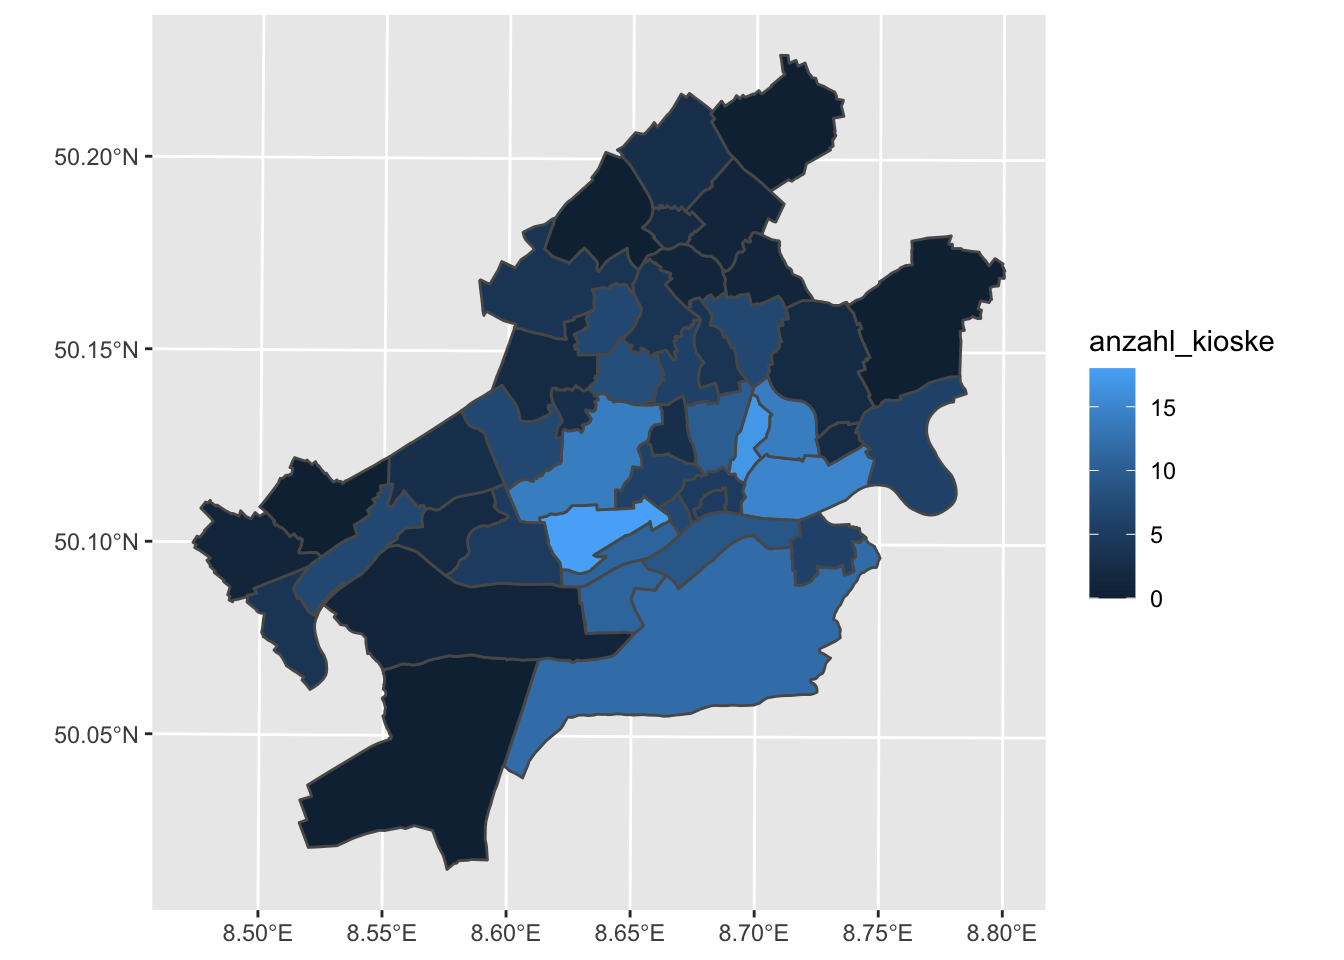
\includegraphics{_main_files/figure-latex/unnamed-chunk-98-1.png}

Zwei Koordinaten sind quatsch! Wir finden ihre ungefähren Werte mit \texttt{summary}:

\begin{Shaded}
\begin{Highlighting}[]
\FunctionTok{summary}\NormalTok{(preise\_geo}\SpecialCharTok{$}\NormalTok{longitude)}
\DocumentationTok{\#\#    Min. 1st Qu.  Median    Mean 3rd Qu.    Max. }
\DocumentationTok{\#\#   5.901   8.021   9.275   9.607  11.058  97.364}
\end{Highlighting}
\end{Shaded}

Und filtern sie raus, und wiederholen die Umwandlung (diesmal auch mit CRS)

\begin{Shaded}
\begin{Highlighting}[]
\NormalTok{preise\_geo }\SpecialCharTok{\%\textgreater{}\%}
  \FunctionTok{filter}\NormalTok{(longitude }\SpecialCharTok{\textless{}} \DecValTok{80}\NormalTok{) }\SpecialCharTok{\%\textgreater{}\%}
  \FunctionTok{st\_as\_sf}\NormalTok{(}\AttributeTok{coords =} \FunctionTok{c}\NormalTok{(}\StringTok{"longitude"}\NormalTok{, }\StringTok{"latitude"}\NormalTok{)) }\SpecialCharTok{\%\textgreater{}\%}
  \FunctionTok{st\_set\_crs}\NormalTok{(}\DecValTok{4326}\NormalTok{) }\OtherTok{{-}\textgreater{}}\NormalTok{ preise\_sf}
\end{Highlighting}
\end{Shaded}

Dann mappen wir nochmal:

\begin{Shaded}
\begin{Highlighting}[]
\FunctionTok{tm\_shape}\NormalTok{(preise\_sf) }\SpecialCharTok{+}
  \FunctionTok{tm\_dots}\NormalTok{(}\StringTok{"dieselpreis"}\NormalTok{, }\AttributeTok{style =} \StringTok{"cont"}\NormalTok{)}
\end{Highlighting}
\end{Shaded}

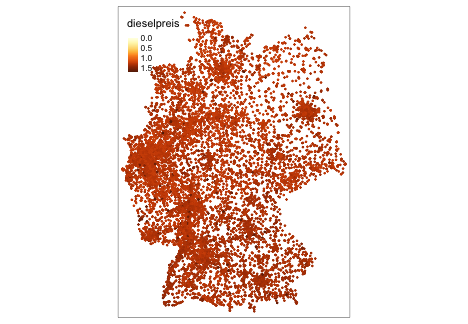
\includegraphics{_main_files/figure-latex/unnamed-chunk-101-1.png}

Schon ganz hübsch, aber die Skala wird nun verzerrt durch sehr teure Autobahntankstellen einerseits, und falsche Null-werte andererseits:

\begin{Shaded}
\begin{Highlighting}[]
\FunctionTok{summary}\NormalTok{(preise\_sf}\SpecialCharTok{$}\NormalTok{dieselpreis)}
\DocumentationTok{\#\#    Min. 1st Qu.  Median    Mean 3rd Qu.    Max. }
\DocumentationTok{\#\#   0.000   1.249   1.289   1.290   1.329   1.679}
\end{Highlighting}
\end{Shaded}

\hypertarget{choroplethen}{%
\subsection{Choroplethen}\label{choroplethen}}

Eine Lösung wäre, die Daten auf Kreisebene zusammenzufassen, und zwar anhand ihres Medians. Damit würden diese Ausreißer keine Role mehr spielen.

Das \texttt{eurostat}-Paket macht es einfach, diese Geodaten einzulesen. NUTS3 ist die Ebene der Stadt- und Landkreise bzw. ihrer europäischen Equivalente.

\begin{Shaded}
\begin{Highlighting}[]
\NormalTok{kreise }\OtherTok{\textless{}{-}}\NormalTok{ eurostat}\SpecialCharTok{::}\FunctionTok{get\_eurostat\_geospatial}\NormalTok{(}\AttributeTok{nuts\_level =} \DecValTok{3}\NormalTok{) }\SpecialCharTok{\%\textgreater{}\%}
  \FunctionTok{filter}\NormalTok{(CNTR\_CODE }\SpecialCharTok{==} \StringTok{"DE"}\NormalTok{)}
\end{Highlighting}
\end{Shaded}

Mal schauen wie es aussieht:

\begin{Shaded}
\begin{Highlighting}[]
\FunctionTok{tm\_shape}\NormalTok{(kreise) }\SpecialCharTok{+}
  \FunctionTok{tm\_polygons}\NormalTok{()}
\end{Highlighting}
\end{Shaded}

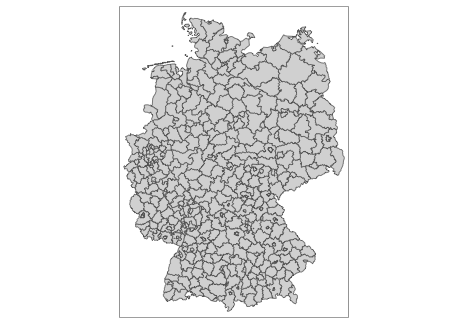
\includegraphics{_main_files/figure-latex/unnamed-chunk-104-1.png}

\hypertarget{ruxe4umliches-verschneiden}{%
\subsection{Räumliches Verschneiden}\label{ruxe4umliches-verschneiden}}

mit \texttt{st\_join} werden Datensätze nicht mit einem Key verschnitten, sondern anhand ihrer Geolokation. Dann können wir wieder ganz normal \texttt{group\_by} und \texttt{summarise} verwenden:

\begin{Shaded}
\begin{Highlighting}[]
\FunctionTok{st\_join}\NormalTok{(kreise, preise\_sf) }\SpecialCharTok{\%\textgreater{}\%}
  \FunctionTok{group\_by}\NormalTok{(NUTS\_ID) }\SpecialCharTok{\%\textgreater{}\%}
  \FunctionTok{summarise}\NormalTok{(}\AttributeTok{dieselpreis =} \FunctionTok{median}\NormalTok{(dieselpreis),}
            \AttributeTok{e5preis     =} \FunctionTok{median}\NormalTok{(e5preis),}
            \AttributeTok{e10preis    =} \FunctionTok{median}\NormalTok{(e10preis)) }\OtherTok{{-}\textgreater{}}\NormalTok{ preise\_kreise}
\end{Highlighting}
\end{Shaded}

Und so könnte vielleicht ein vorläufiges Ergebnis aussehen:

\begin{Shaded}
\begin{Highlighting}[]
\FunctionTok{tm\_shape}\NormalTok{(preise\_kreise) }\SpecialCharTok{+}
  \FunctionTok{tm\_fill}\NormalTok{(}\StringTok{"dieselpreis"}\NormalTok{,}
          \AttributeTok{title =} \StringTok{"Median der Dieselpreise"}\NormalTok{,}
          \AttributeTok{style =} \StringTok{"cont"}\NormalTok{,}
          \AttributeTok{alpha =} \FloatTok{0.8}\NormalTok{) }\SpecialCharTok{+}
  \FunctionTok{tm\_layout}\NormalTok{(}\AttributeTok{legend.outside =} \ConstantTok{TRUE}\NormalTok{)}
\end{Highlighting}
\end{Shaded}

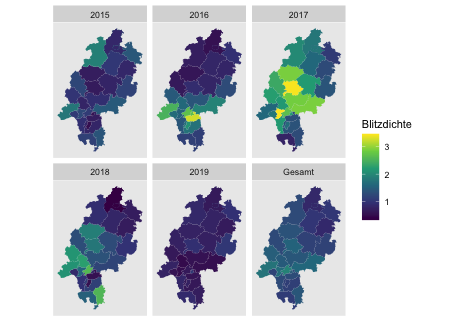
\includegraphics{_main_files/figure-latex/unnamed-chunk-106-1.png}

\hypertarget{publizieren-und-nach-hilfe-fragen}{%
\section{Publizieren und nach Hilfe fragen}\label{publizieren-und-nach-hilfe-fragen}}

\hypertarget{publizieren-mit-rmarkdown}{%
\subsection{Publizieren mit Rmarkdown}\label{publizieren-mit-rmarkdown}}

\hypertarget{text-formatieren}{%
\subsubsection{Text formatieren}\label{text-formatieren}}

Wir arbeiten schon von Anfang an mit im Rmarkdown-Format. Wie Überschriften, Links, Bilder usw. in Rmarkdown genau funktionieren, ist in \href{https://rmarkdown.rstudio.com/authoring_basics.html}{dieser Übersicht} und auf \href{https://github.com/rstudio/cheatsheets/blob/master/rmarkdown-2.0.pdf}{diesem Cheat Sheet} gut festgehalten.

\hypertarget{der-knit-button}{%
\subsubsection{Der Knit-Button}\label{der-knit-button}}

Wenn wir im \href{https://de.wikipedia.org/wiki/YAML}{YAML}-Header die Zeile

\begin{verbatim}
output: html_document
\end{verbatim}

setzen, erscheint (nach Abspeichern) ein „Knit``-Button in der GUI. Durch Drücken auf diesen Knopf passiert folgendes:

\begin{itemize}
\tightlist
\item
  R erstellt („strickt``) ein HTML-Dokument aus dem vorliegenden Markdown und den Code Chunks
\item
  Dabei spielen „gespeicherte`` Objekte keine Rolle, die Chunks werden einfach der Reihe nach (in einem neuen Environment) ausgeführt
\item
  Externe Datensätze o.~ä. müssen also am Anfang des Dokuments explizit geladen werden (etwa mit \texttt{load()}). Für den Abschlussbericht ist es ratsam, einen vorbereiteten Datensatz am Anfang des Rmarkdown-Dokuments so zu laden.
\end{itemize}

Im YAML-Header können noch viele weitere Angaben gemacht werden, die das Resultat verändern. Hier eine gute Dokumentation: \url{https://bookdown.org/yihui/rmarkdown/html-document.html}

\hypertarget{kable}{%
\subsubsection{Kable}\label{kable}}

Im \texttt{knitr}-Paket sorgt der Befehl \texttt{kable()} für eine schöne Darstellung von Tabellen:

\begin{Shaded}
\begin{Highlighting}[]
\NormalTok{ggplot2}\SpecialCharTok{::}\NormalTok{diamonds }\SpecialCharTok{\%\textgreater{}\%}
  \FunctionTok{head}\NormalTok{() }\SpecialCharTok{\%\textgreater{}\%}
\NormalTok{  knitr}\SpecialCharTok{::}\FunctionTok{kable}\NormalTok{()}
\end{Highlighting}
\end{Shaded}

\begin{tabular}{r|l|l|l|r|r|r|r|r|r}
\hline
carat & cut & color & clarity & depth & table & price & x & y & z\\
\hline
0.23 & Ideal & E & SI2 & 61.5 & 55 & 326 & 3.95 & 3.98 & 2.43\\
\hline
0.21 & Premium & E & SI1 & 59.8 & 61 & 326 & 3.89 & 3.84 & 2.31\\
\hline
0.23 & Good & E & VS1 & 56.9 & 65 & 327 & 4.05 & 4.07 & 2.31\\
\hline
0.29 & Premium & I & VS2 & 62.4 & 58 & 334 & 4.20 & 4.23 & 2.63\\
\hline
0.31 & Good & J & SI2 & 63.3 & 58 & 335 & 4.34 & 4.35 & 2.75\\
\hline
0.24 & Very Good & J & VVS2 & 62.8 & 57 & 336 & 3.94 & 3.96 & 2.48\\
\hline
\end{tabular}

Auch hier gibt es wieder vielfältige Möglichkeiten zur visuellen Gestaltung. Diesen Post finde ich immer besonders hilfreich: \url{https://haozhu233.github.io/kableExtra/awesome_table_in_html.html}

\hypertarget{chunk-options}{%
\subsubsection{Chunk Options}\label{chunk-options}}

Am Anfang eines Code Chunks kann genau festgelegt werden, ob der Code ausgeführt werden soll, ob er im finalen Dokument erscheinen soll, ob Warnungen oder Fehler ausgegeben werden sollen, etc. Wenn zum Beispiel Libraries „versteckt`` geladen werden sollen, geht das mit diesem Code Chunk:

\begin{verbatim}
```{r, include = FALSE}
library(tidyverse)
library(rvest)
```
\end{verbatim}

Ein überblick über die Chunk-Optionen findet sich hier: \url{https://bookdown.org/yihui/rmarkdown/r-code.html}

\hypertarget{reproducible-research}{%
\subsubsection{Reproducible research}\label{reproducible-research}}

Wenn z.~B. ein (längeres) Script einen (größeren) Datensatz generiert und ihn dem Objektnamen \texttt{mein\_datensatz} zuweist, dann erscheint der Datensatz im lokalen Environment. Um den Datensatz mit anderen zu teilen, muss er irgendwie exportiert werden. Hierfür ist es ratsam, die \texttt{save()}-Funktion zu nutzen:

\begin{Shaded}
\begin{Highlighting}[]
\FunctionTok{save}\NormalTok{(mein\_datensatz, }\AttributeTok{file =} \StringTok{"zwischenstand\_mein\_datensatz.Rdata"}\NormalTok{)}
\end{Highlighting}
\end{Shaded}

So wird eine Datei erstellt, die den Datensatz enthält und verschoben oder geteilt werden kann. Eine solche Datei kann auch andere Objekte (Funktionen, Listen, \ldots) und mehrere Objekte auf einmal enthalten. Die Dateiendung ist dabei eigentlich egal, \texttt{.Rdata} scheint aber Usus zu sein.

Aus der Datei können Objekte dann jederzeit wieder ins Environment geladen werden mit dem Befehl:

\begin{Shaded}
\begin{Highlighting}[]
\FunctionTok{load}\NormalTok{(}\StringTok{"zwischenstand\_mein\_datensatz.Rdata"}\NormalTok{)}
\end{Highlighting}
\end{Shaded}

Auch wenn ein Skript auf einmal nicht mehr funktioniert (etwa weil die API sich ändert), ist es hilfreich, auf solche Zwischenstände zurückgreifen zu können.

\hypertarget{wissenschaftliches-zitieren}{%
\subsubsection{Wissenschaftliches Zitieren}\label{wissenschaftliches-zitieren}}

Wer die Vorzüge von Literaturverwaltungssoftware (wie Citavi, Zotero, \ldots) schon schätzen gelernt hat, kann in Rmarkdown folgendermaßen vorgehen:

\hypertarget{schritt-1-exportieren}{%
\paragraph{Schritt 1: Exportieren}\label{schritt-1-exportieren}}

Die relevante Literatur in eine BibTex-Datei im R-Arbeitsverzeichnis exportieren, z.B. \texttt{literatur.bib}. BibTex (bzw. BibLatex) ist ein bewährtes und gut dokumentiertes Format. Ein Eintrag sieht dann z.B. so aus, wobei \texttt{bortz} der „Name`` des Eintrags ist, den wir frei wählen können:

\begin{verbatim}
@book{bortz,
  author = {Bortz, J{\"u}rgen and Schuster, Christof},
  title = {{Statistik f{\"u}r Human- und Sozialwissenschaftler}},
  publisher = {Springer},
  year = {2010},
  address = {Berlin},
  edition = {7},
}
\end{verbatim}

\hypertarget{schritt-2-verlinken}{%
\paragraph{Schritt 2: Verlinken}\label{schritt-2-verlinken}}

Im YAML-Header des Rmarkdown-dokuments die Angabe ergänzen:

\begin{verbatim}
bibliography: literatur.bib
\end{verbatim}

Damit weiß der „Knit``-Befehl, wo er nach Literatur suchen soll.

\hypertarget{schritt-3-zitieren}{%
\paragraph{Schritt 3: Zitieren}\label{schritt-3-zitieren}}

Im Text kann dann z.~B. so zitiert werden:

\begin{verbatim}
Das zentrale Grenzwerttheorem besagt, dass die Stichprobenverteilung von
$\bar{x}$ mit steigender Stichprobengröße $n$ in eine Normalverteilung übergeht
[@bortz: 86].
\end{verbatim}

\hypertarget{schritt-4-stricken}{%
\paragraph{Schritt 4: Stricken}\label{schritt-4-stricken}}

Beim „Knit``-Befehl wird ein Literaturverzeichnis automatisch erstellt und ans Ende des Dokuments gehängt. Deshalb beendet man das Dokument am besten mit der Zeile:

\begin{verbatim}
## Literaturverzeichnis
\end{verbatim}

\hypertarget{nach-hilfe-fragen}{%
\subsection{Nach Hilfe fragen}\label{nach-hilfe-fragen}}

Online-Foren, insb. \href{https://stackoverflow.com}{Stackoverflow} sind tolle Ressourcen um Probleme beim Programmieren zu lösen. (Weniger bekannt: die Statistik-Schwesterseite \href{https://stats.stackexchange.com}{Cross Validated}.)

Oft landet man auf Stackoverflow, wenn man nach einer Fehlermeldung oder einer Problemstellung googelt. Aber obwohl die Stackoverflow-Community den Ruf hat, sehr streng zu sein und Hilfegesuche einfach ``abzubügeln'', ist es gar nicht so verkehrt hier nach Hilfe auch zu komplexen Problemen zu fragen.

Um hilfreiches Feedback zu bekommen, lohnt es sich jedoch, einige Punkte zu beachten:

\begin{itemize}
\tightlist
\item
  Fragen können mit Stichworten getaggt werden. Neben dem Tag ``R'' lohnt es sich, konkrete Pakete wie ``ggplot2'', ``sf'' o.~ä. zu taggen, damit die ``richtigen'' Personen darauf aufmerksam werden.
\item
  Ein ganz kurzer einleitender Satz zum Kontext sollte nicht fehlen: ``I'm trying to \ldots{} in order to \ldots{}''
\item
  Wenn es eine existierende Frage oder eine Online-Ressource gibt, die dem Problem sehr ähnlich ist (aber nicht ganz auf den Fall passt), ist es ratsam darauf zu verweisen: ``I already tried this solution, but my problem is \ldots{}''
\item
  \href{https://en.wikipedia.org/wiki/Minimal_working_example}{Kurze, reproduzierbare Beispiele} helfen den Antwortenden dabei, mögliche Lösungen auszuprobieren und zu testen.
\item
  Dabei ist es oft sinnvoll, kurze Auszüge von Datensätzen in die Frage einzubauen -- und zwar so, dass sie einfach in R kopiert werden können. Das geht oft ganz gut mit \texttt{dput(head(DATENSATZ))}. Weitere Infos dazu: \url{https://stackoverflow.com/questions/5963269/how-to-make-a-great-r-reproducible-example\#5963610}
\item
  Schließlich ist es hilfreich deutlich zu machen, was das unmittelbare Ziel des Codes ist: ``My expected output should look like this: \ldots{}''
\end{itemize}


\end{document}
